\title{Note on estimating the error of the extracted time resolution of the FTOF12 panel 1b using the automated 6-bar analysis program
error analysis of the extracted time resolution using the automated 6-bar analysis program}
\date{July 05, 2015}

\documentclass[12pt]{article}

\usepackage{hyperref}
\usepackage{cite}

\usepackage{graphicx}
\usepackage{epsfig}
\usepackage{epstopdf}

\usepackage[pdf]{pstricks}

\usepackage{mathtools}
\newcommand{\defeq}{\vcentcolon=}

\usepackage{float}
\restylefloat{table}

%! To create a place-holder figure
\newcommand{\dummyfig}[1]{
  \centering
  \fbox{
    \begin{minipage}[c][0.33\textheight][c]{0.5\textwidth}
      \centering{#1}
    \end{minipage}
  }
}

\begin{document}
\maketitle

% \begin{abstract}
% This is the paper's abstract \ldots
% \end{abstract}

 
\section{Introduction}

Estimating the true error of the extracted time resolution of the system requires a thorough analysis of the statistical and non-statistical uncertainties. Given the scale of the project and therefore, constraints on the time it was not possible to, during production, estimate even the true statistical error of the system. In this section is described the method that was used post production using a set of reference counters -- 6x210cm bars(half slow, half fast) and 1st article PMTs -- to estimate the true statistical error for 210cm counters and then extrapolate them to bars of all lengths. This extrapolation also includes the effect of non-statistical sources of errors in the measurement, for example those pertaining to the physical properties of the counters themselves. 

Before describing the method and showing the results, the manifestation of the time constraint on the measurement and analysis procedure during the production phase and how it affected the extraction of the error on the finally obtained time resolution --with particular attention to it interpreting some key plots-- during this phase are described in the following sub sections.

\subsection{Limited statistics in 6-bar-method measurements}
For each bar length even after 2 days of data taking the statistics in the T histogram (\textit{refer to formula in doc.}) are low and therefore, the statistical methods that can be used to fit and obtain the standard deviation of these histograms, which is the time resolution, has to be studied since each method, in the low statistic limit, has its own limitation in estimating the true standard deviation and its error. 

Figure 1. shows the statistics accumulated (N) for the shortest and longest counters versus points along the bar. Figures 2. and 3. show a comparison of the various fitting methods available in ROOT for extracting $\mu$ and $\sigma$ from simulated Gaussian histograms ($\mu_{T}$ and $\sigma_{T}$) for N values between 100 and 600, reflecting the low and high end of the statistics versus bar length (as can be seen in Figure 1.). The range of simulated $\sigma_{T}$, similarly, covers the low and high end of the typical standard deviation values expected from the FTOF12 system, corresponding to the shortest and longest bars, respectively (\textit{confirm this!}).

\begin{figure*}[ht]
	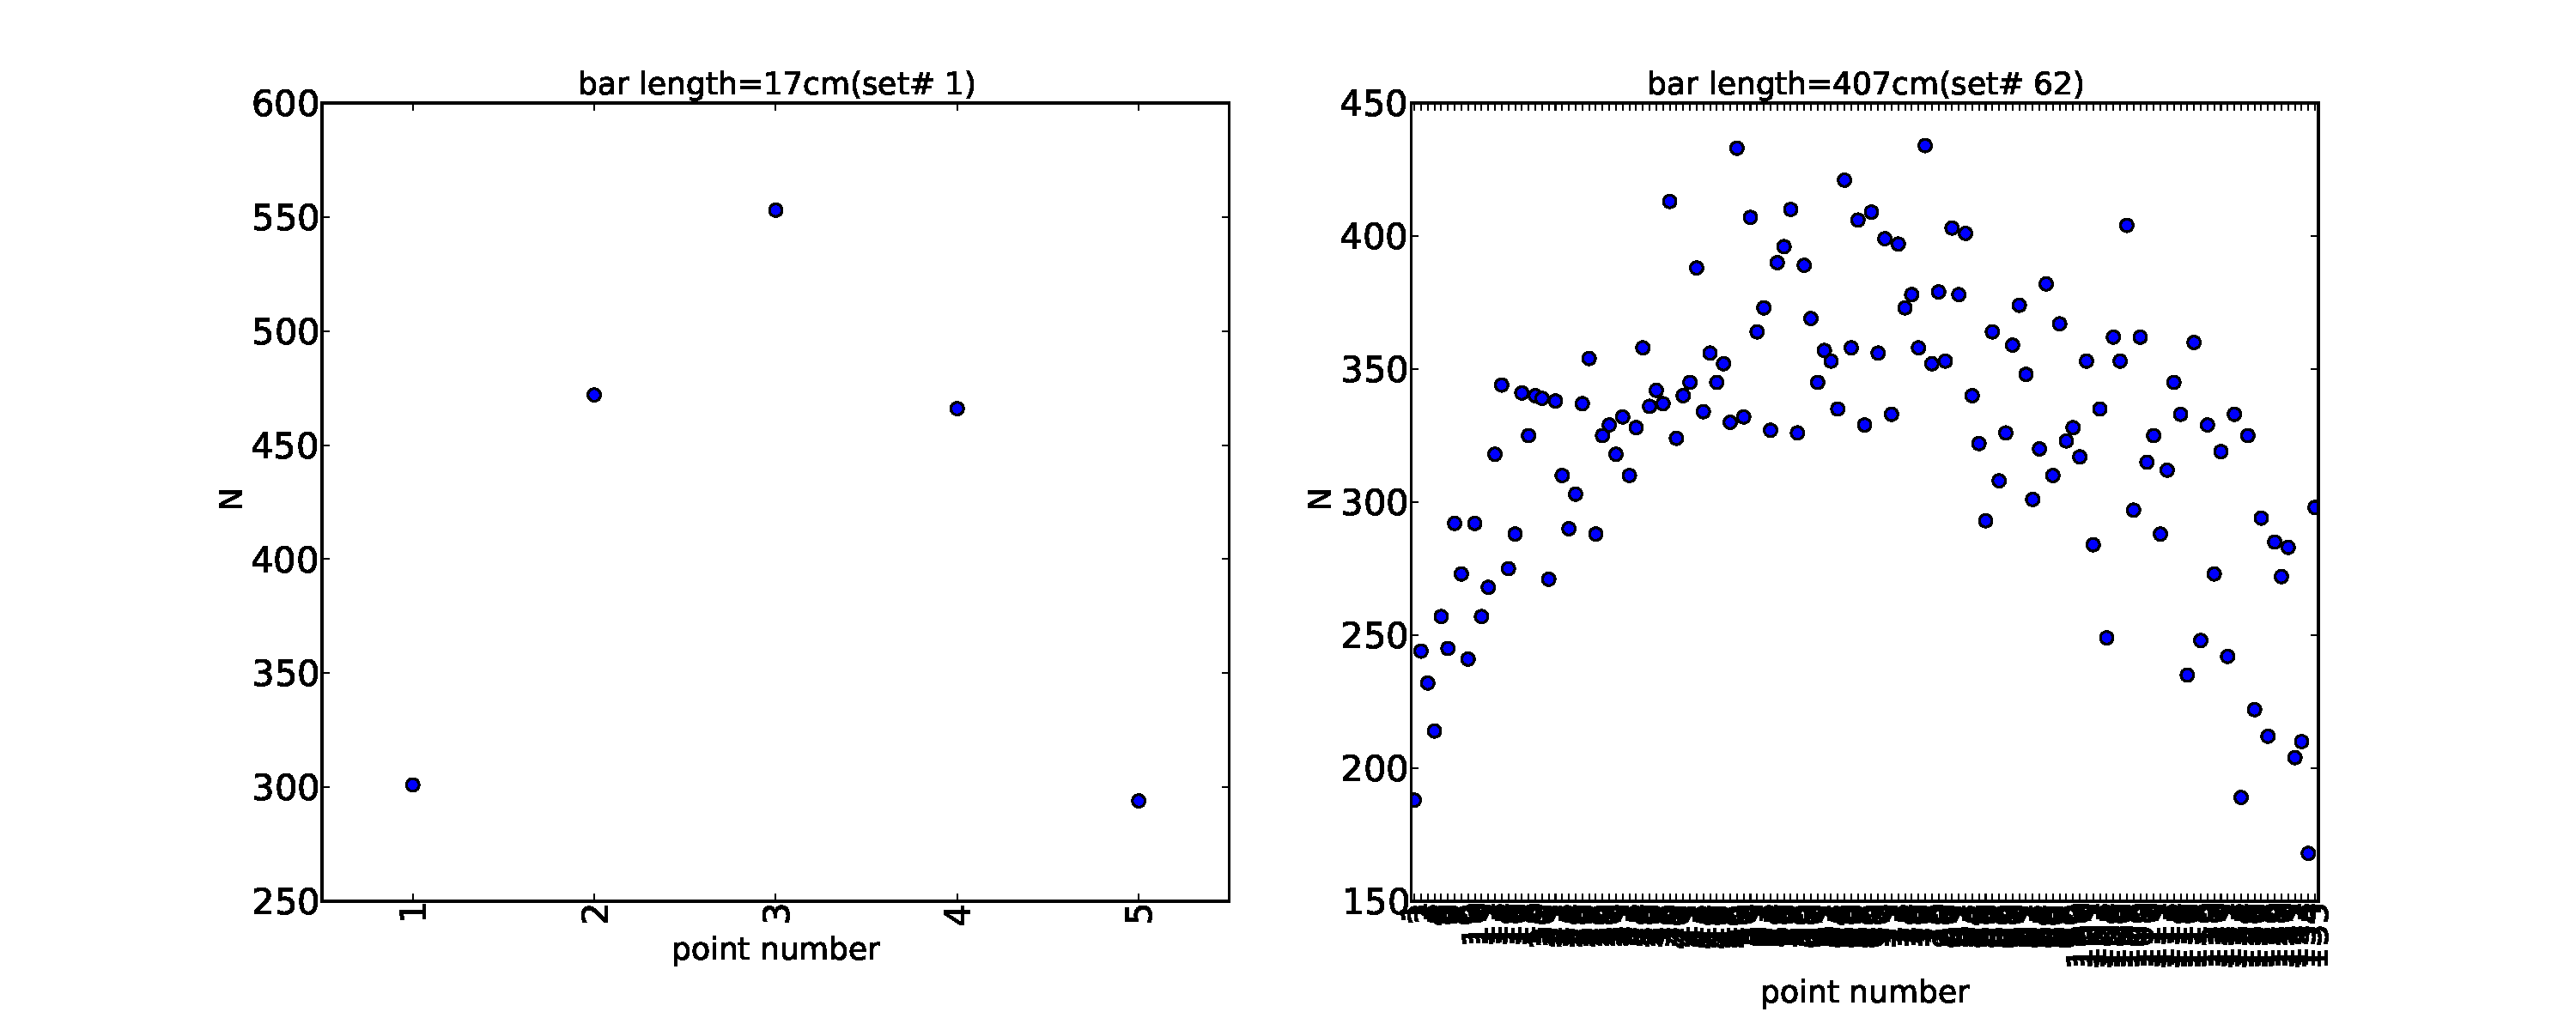
\includegraphics[height=2in,width=5in]{bar_stats_write-up_N-vs-p.pdf}
	\caption{N vs. P for the shortest and longest counters}
	\label{fig1}
\end{figure*}

Figure 2. is a comparison of the Chi-square(CSQ) method with Maximum Likelihood(MLE). It is observed that as the ratio of $\frac{\sigma_{T}}{N}$ gets higher i.e. the entries per bin in the simulated T-histogram decreases, the accuracy of the estimated $\sigma_{T}$ and the error on the estimate reaches unacceptable levels for CSQ. The MLE estimate while significantly better, does tend to underestimate $\sigma_{T}$ by $\approx$ 1\%. In comparison, the estimated $\mu_{T}$ from both methods is similar, except when $\frac{\sigma_{T}}{N}$ reaches its upper most limit, where MLE, again, dominates. Only in the high N limit -- note a discontinuity in the x axis at N=600, after which the values approach the high N limit -- do the two methods begin to converge, but still not completely.

While this observation clearly establishes the superiority of the MLE method in the low N limit, it is not suited for our purpose because it is highly susceptible to data points that are ``outliers'' and appear only in the measured T-distribution. Such ``outliers'' are far and few, yet affect the MLE method and make it estimate a higher standard deviation. The other remaining option is to use a modified version of the CSQ fit in ROOT (CSQ-WW) where, effectively, the error bars in the histogram bins are ignored(\textit{Confirm this at the code level in ROOT and if indeed the documentation in ROOT for WW, ``set weights in all bins to 1;ignore error bars'' means this}). which behaves like MLE, but it is slightly more biased in its estimation of $\sigma_{T}$ for low N, $\approx$ 2\% understimation of $\sigma_{T}$, and the error on this estimate is lower. Fig. 3 shows the extracted parameters from the CSQ-WW option (compared with CSQ)

\begin{figure*}[ht]
	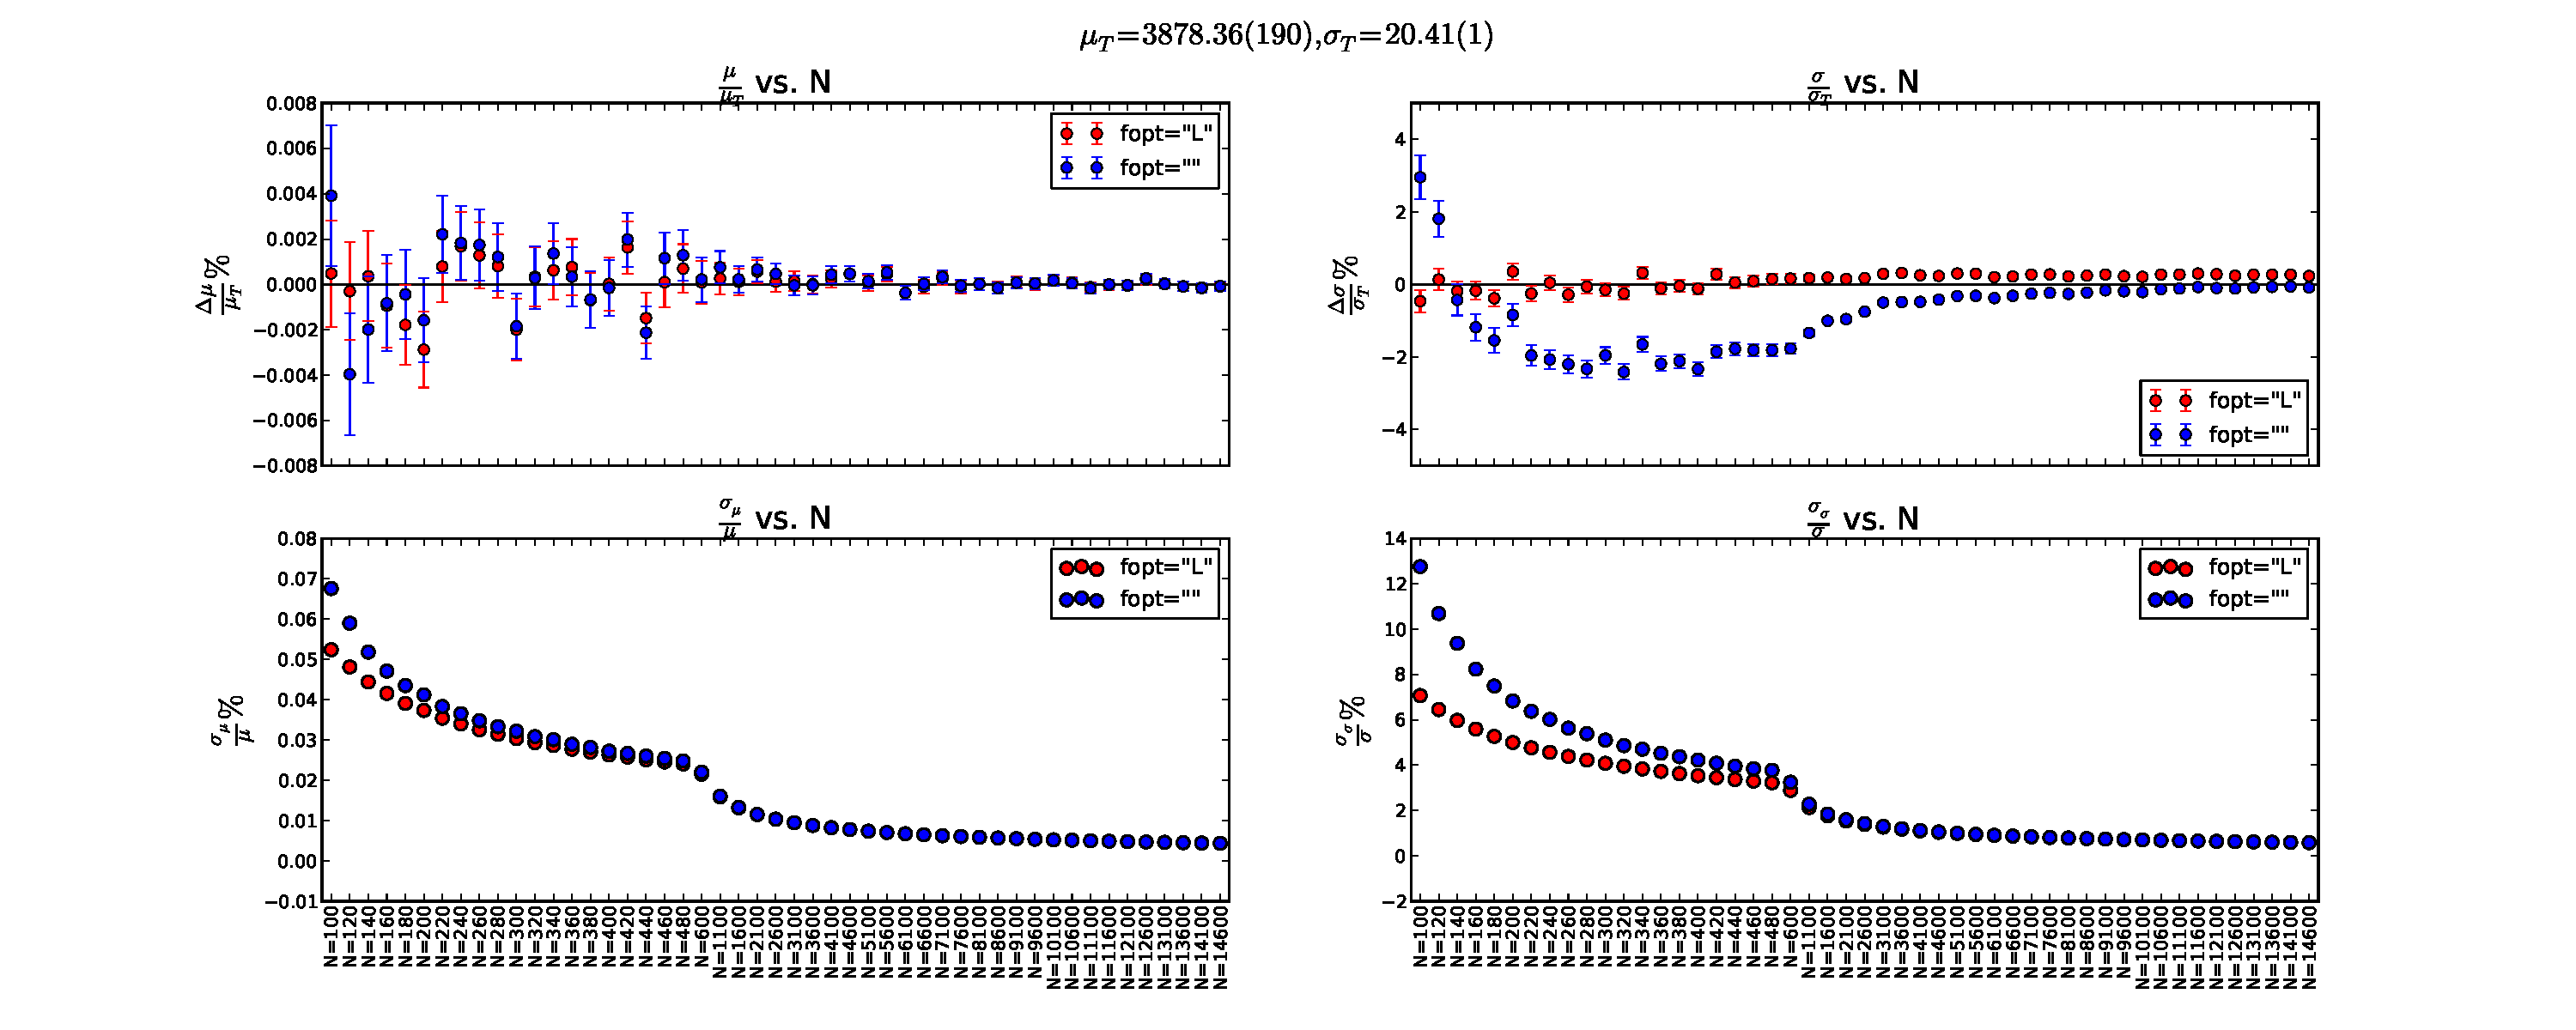
\includegraphics[height=2.5in,width=5.5in]{fit-comp_MU-190_SG-1_fit-opt-L_binw-025.pdf}
	%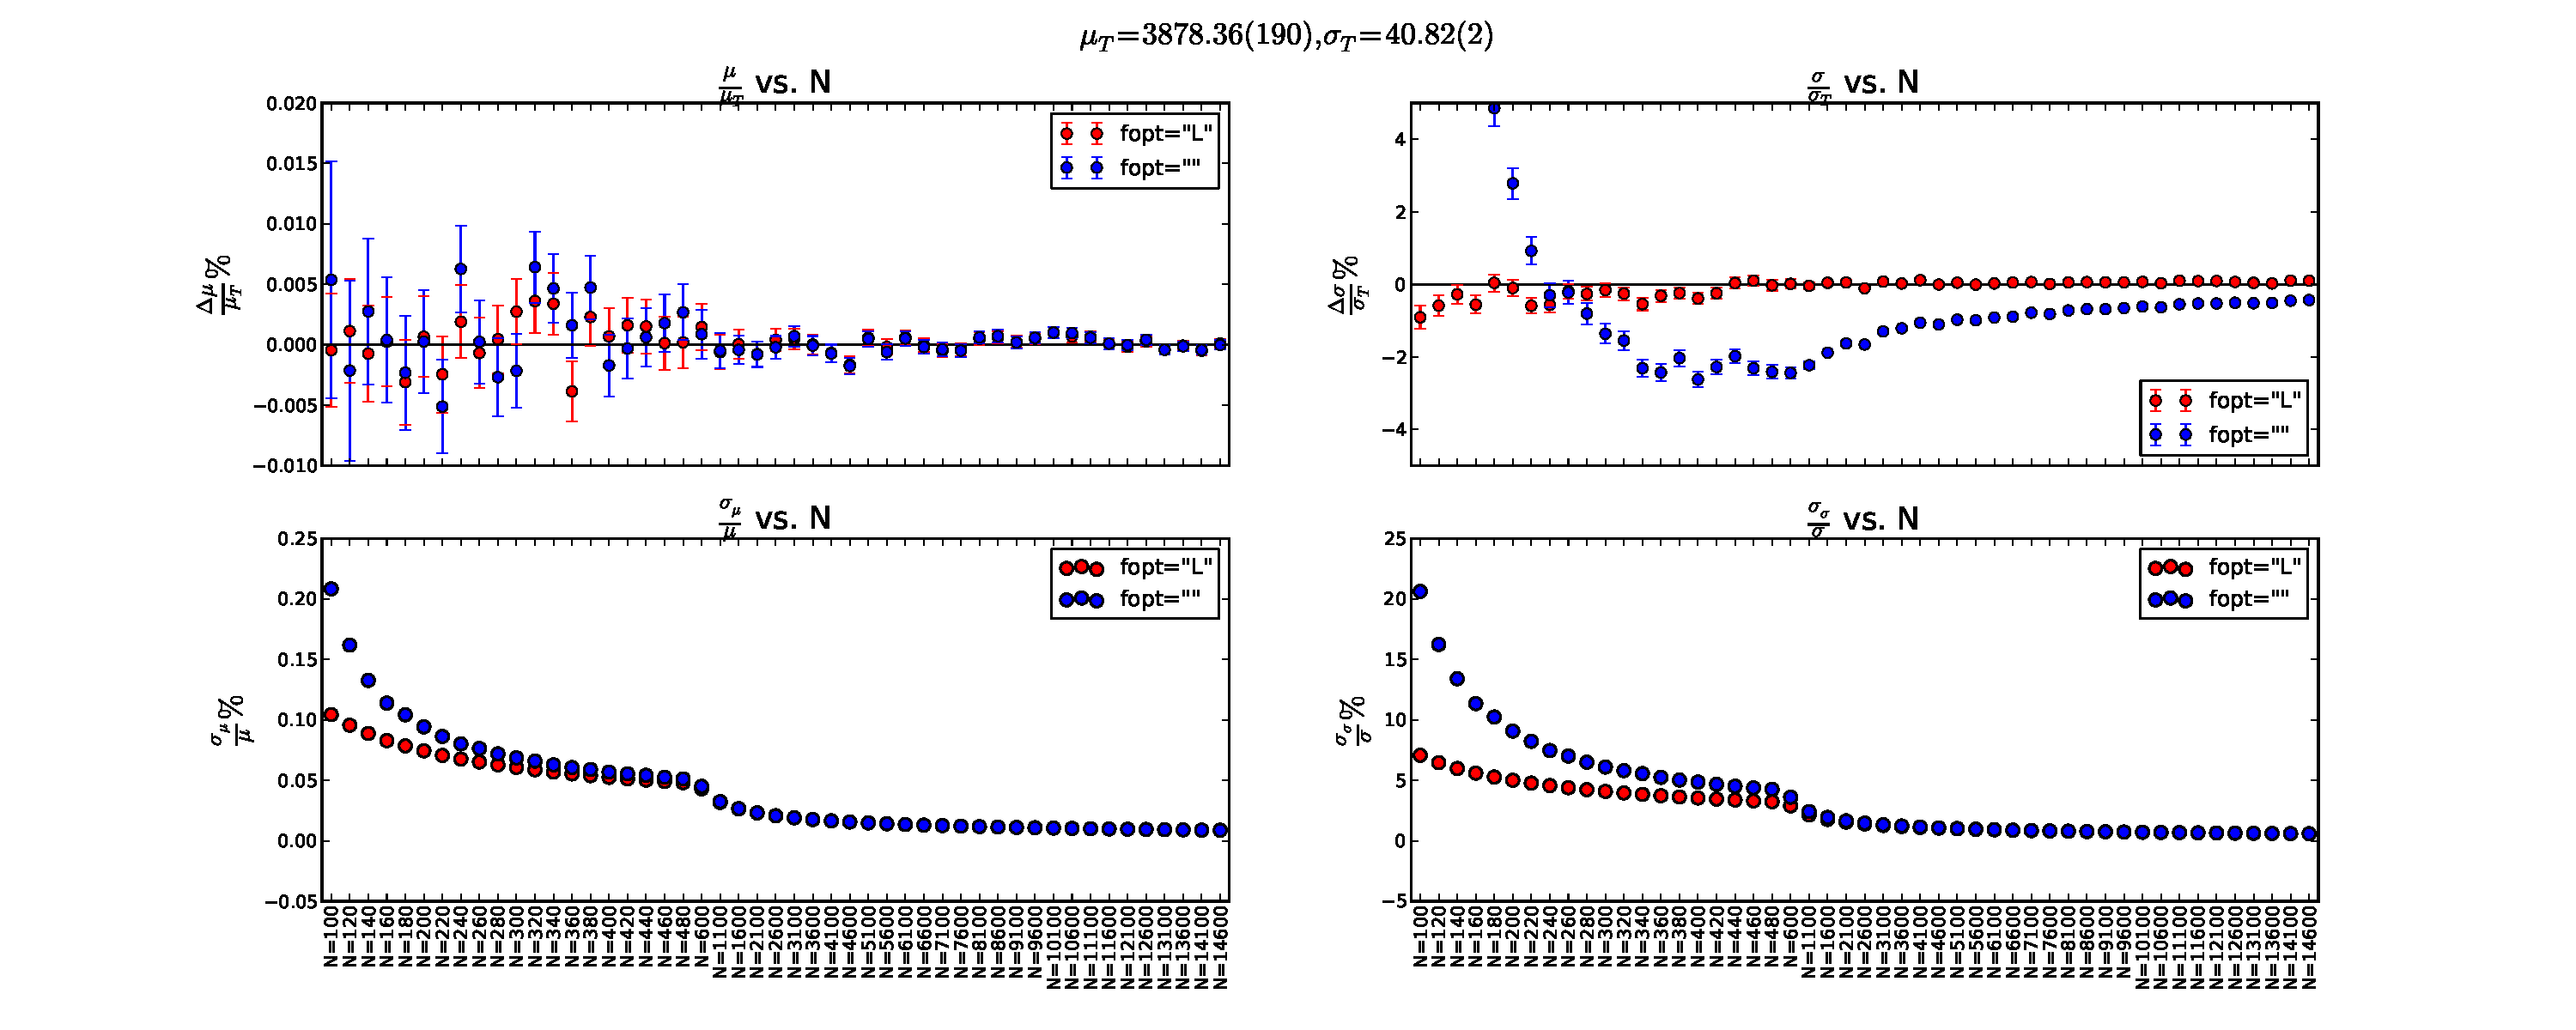
\includegraphics[height=2.5in,width=5.5in]{fit-comp_MU-190_SG-2_fit-opt-L_binw-025.pdf}
	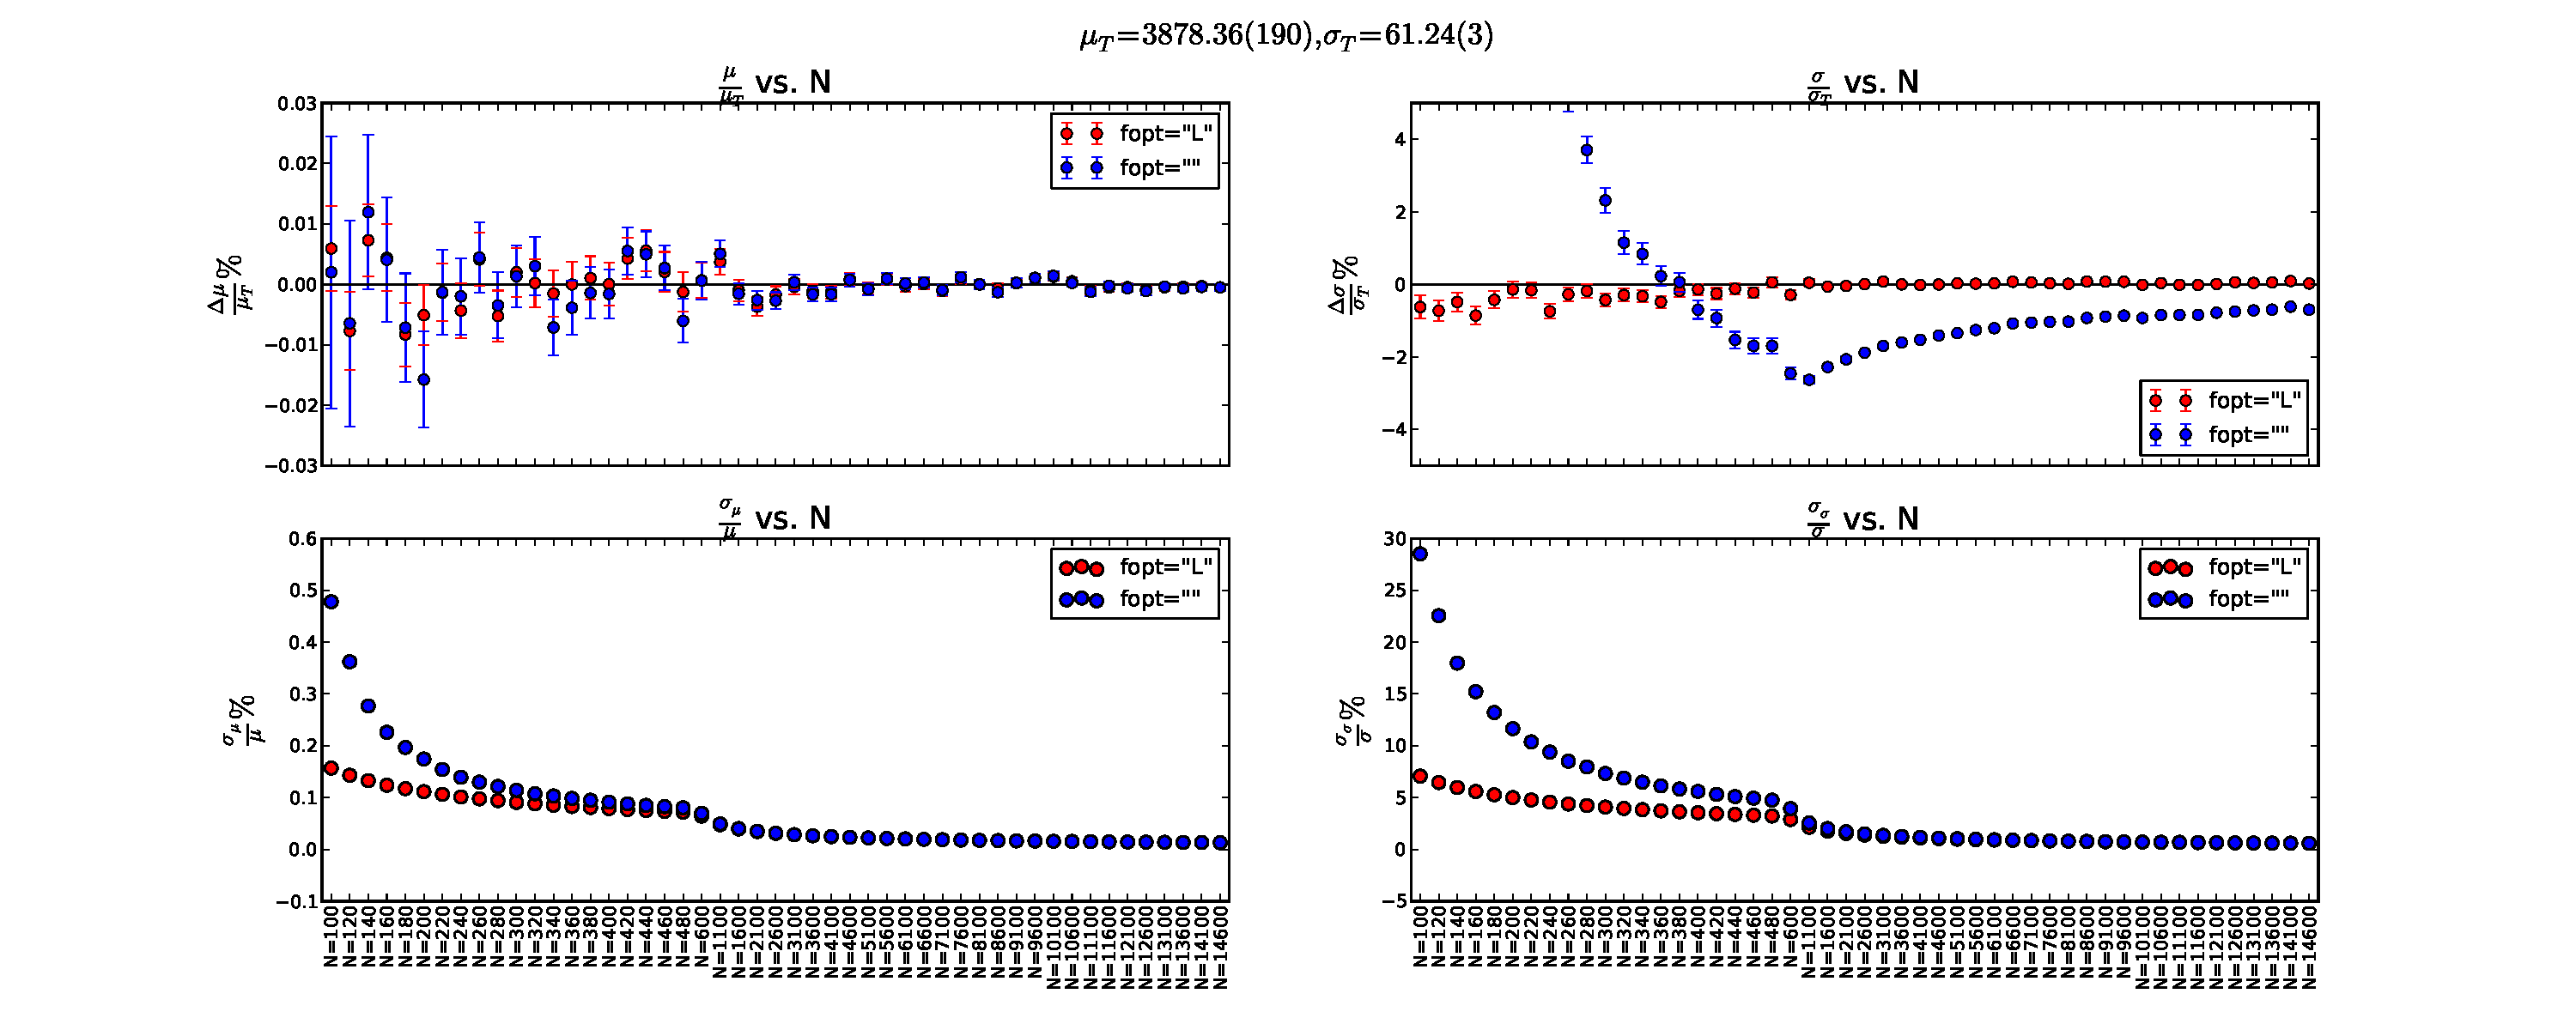
\includegraphics[height=2.5in,width=5.5in]{fit-comp_MU-190_SG-3_fit-opt-L_binw-025.pdf}
	%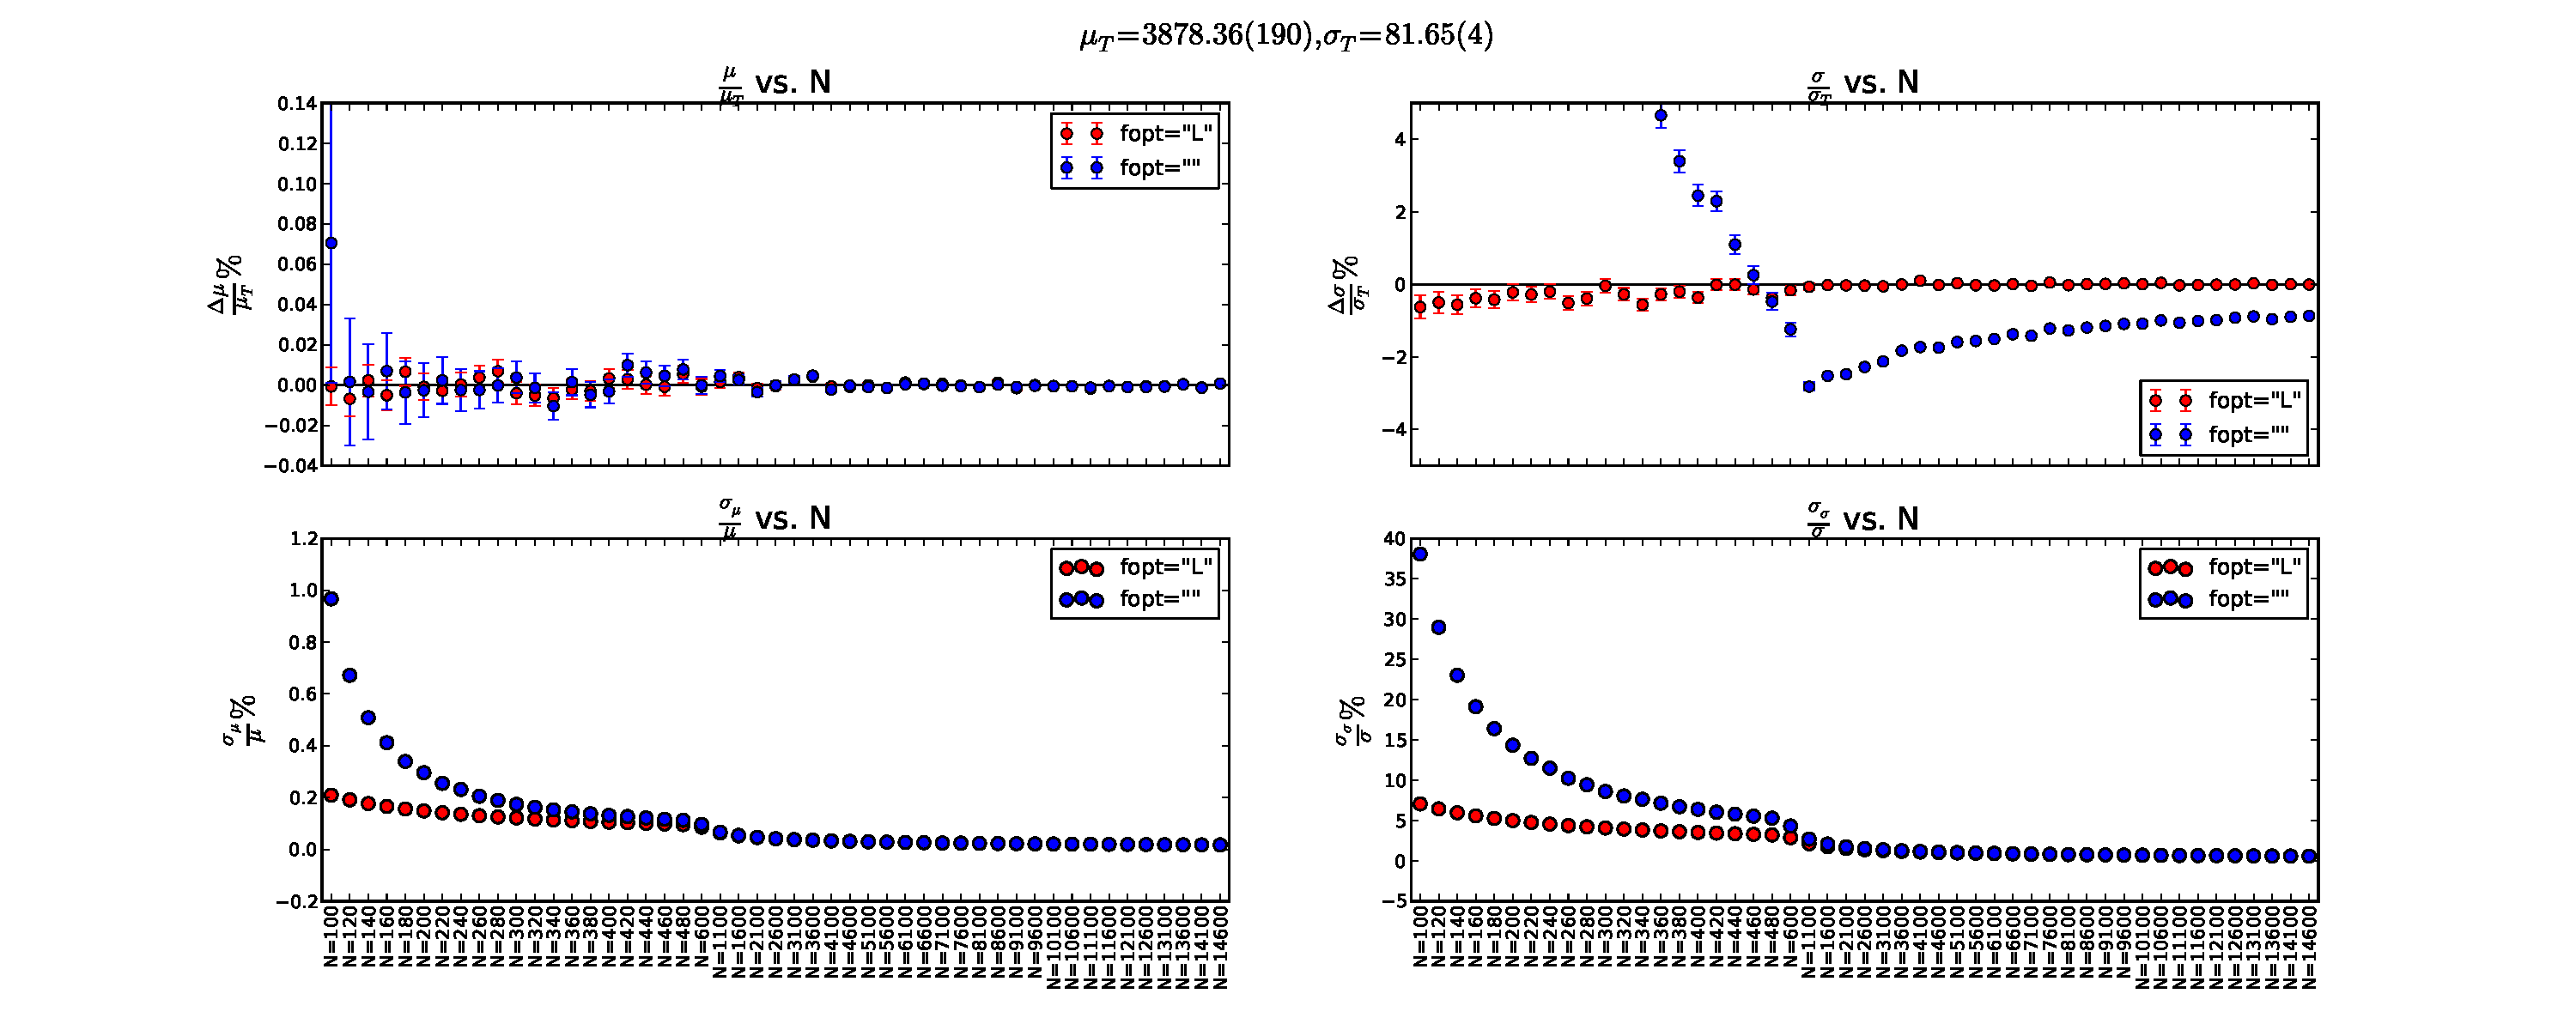
\includegraphics[height=2.5in,width=5.5in]{fit-comp_MU-190_SG-4_fit-opt-L_binw-025.pdf}
	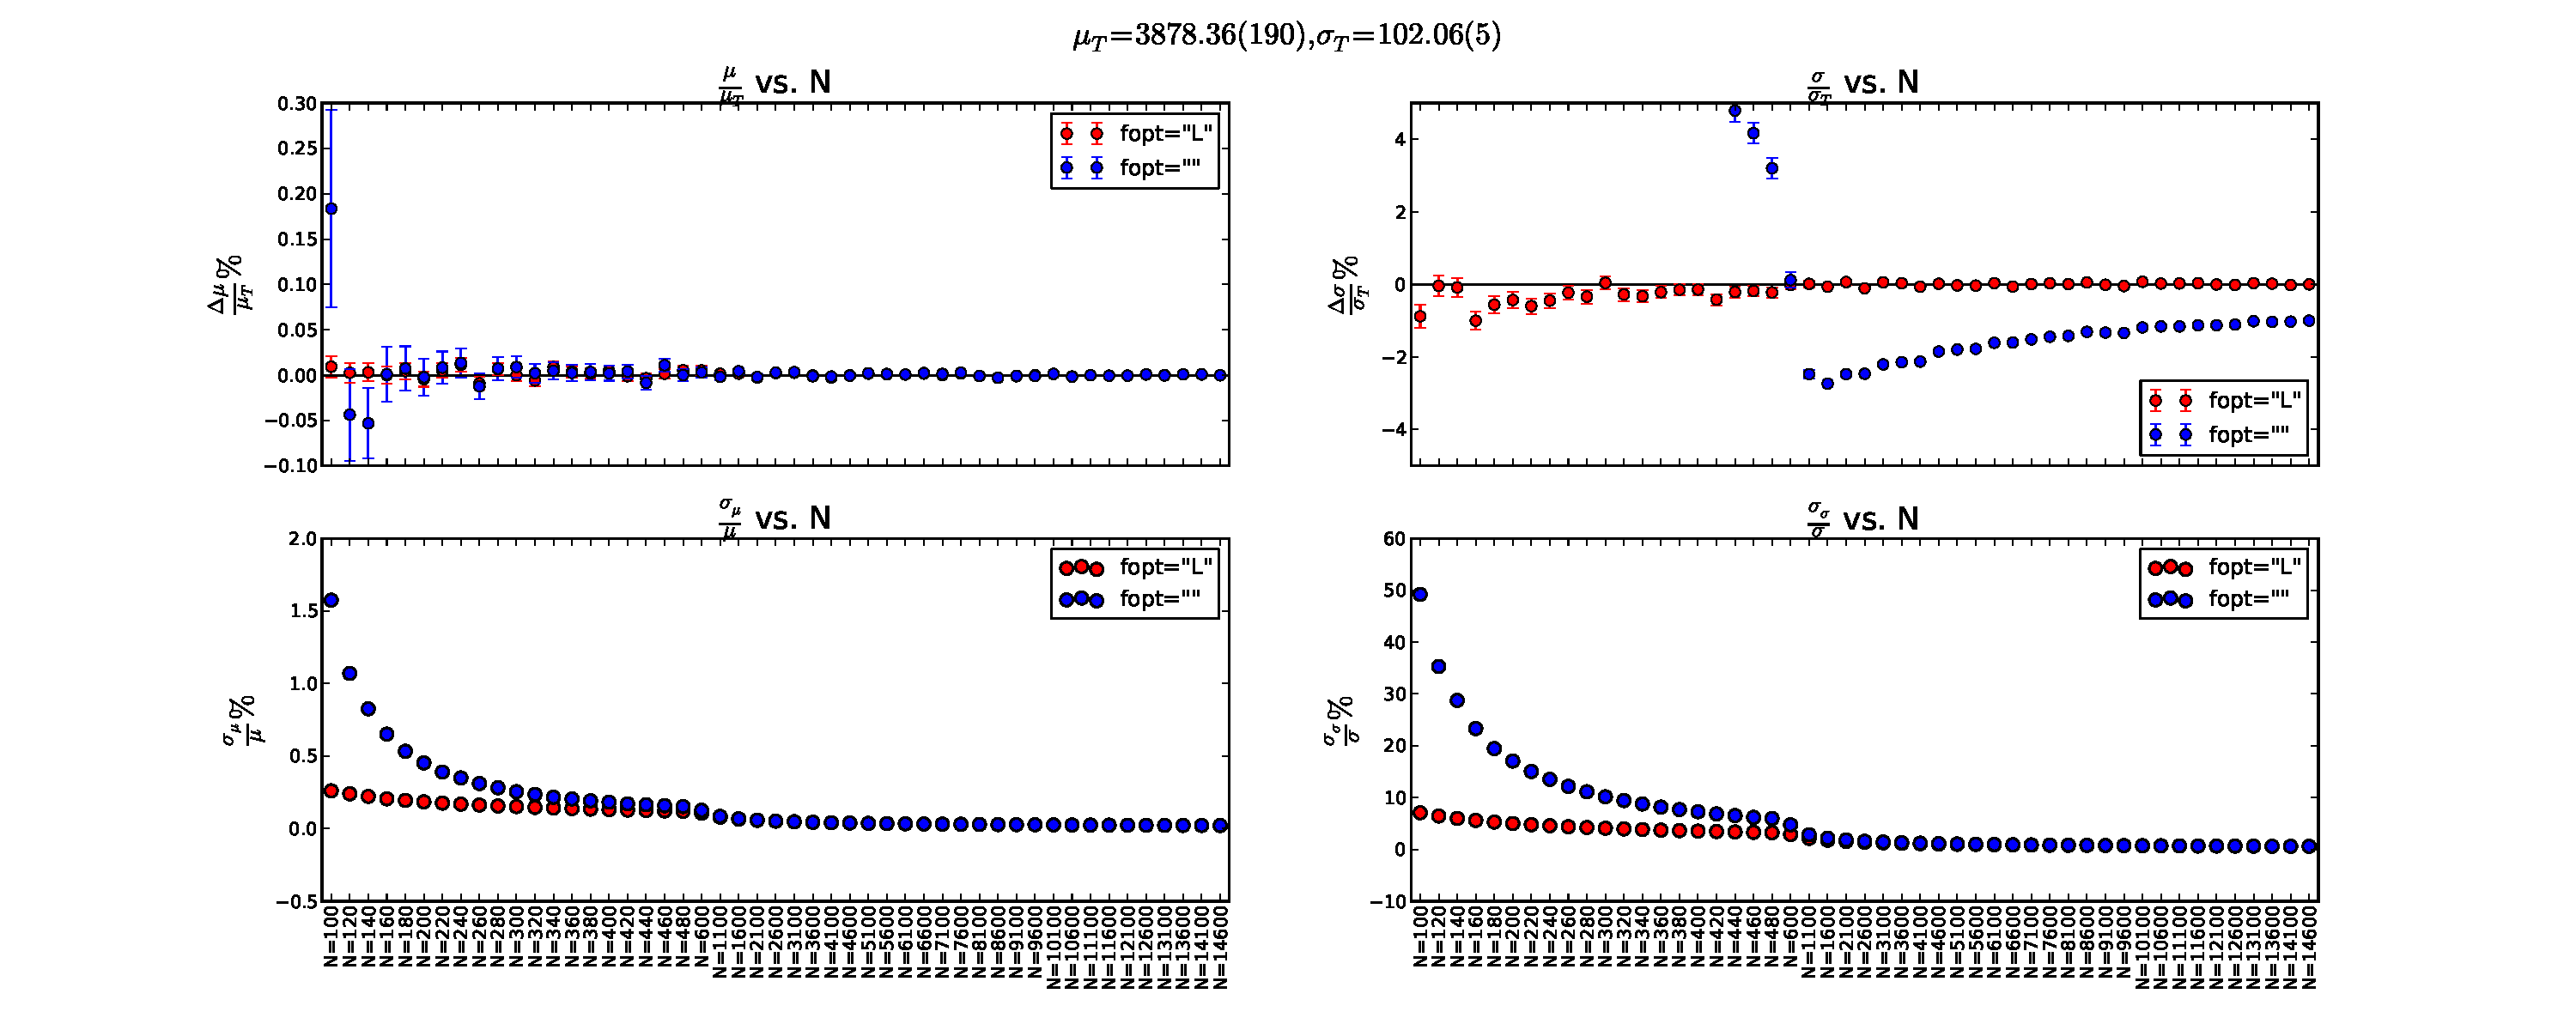
\includegraphics[height=2.5in,width=5.5in]{fit-comp_MU-190_SG-5_fit-opt-L_binw-025.pdf}
	\caption{Extracted parameters (MLE and CSQ) as a function of N and $\sigma_{T}$}
	\label{fig2}
\end{figure*}

\clearpage

\begin{figure*}[ht]
	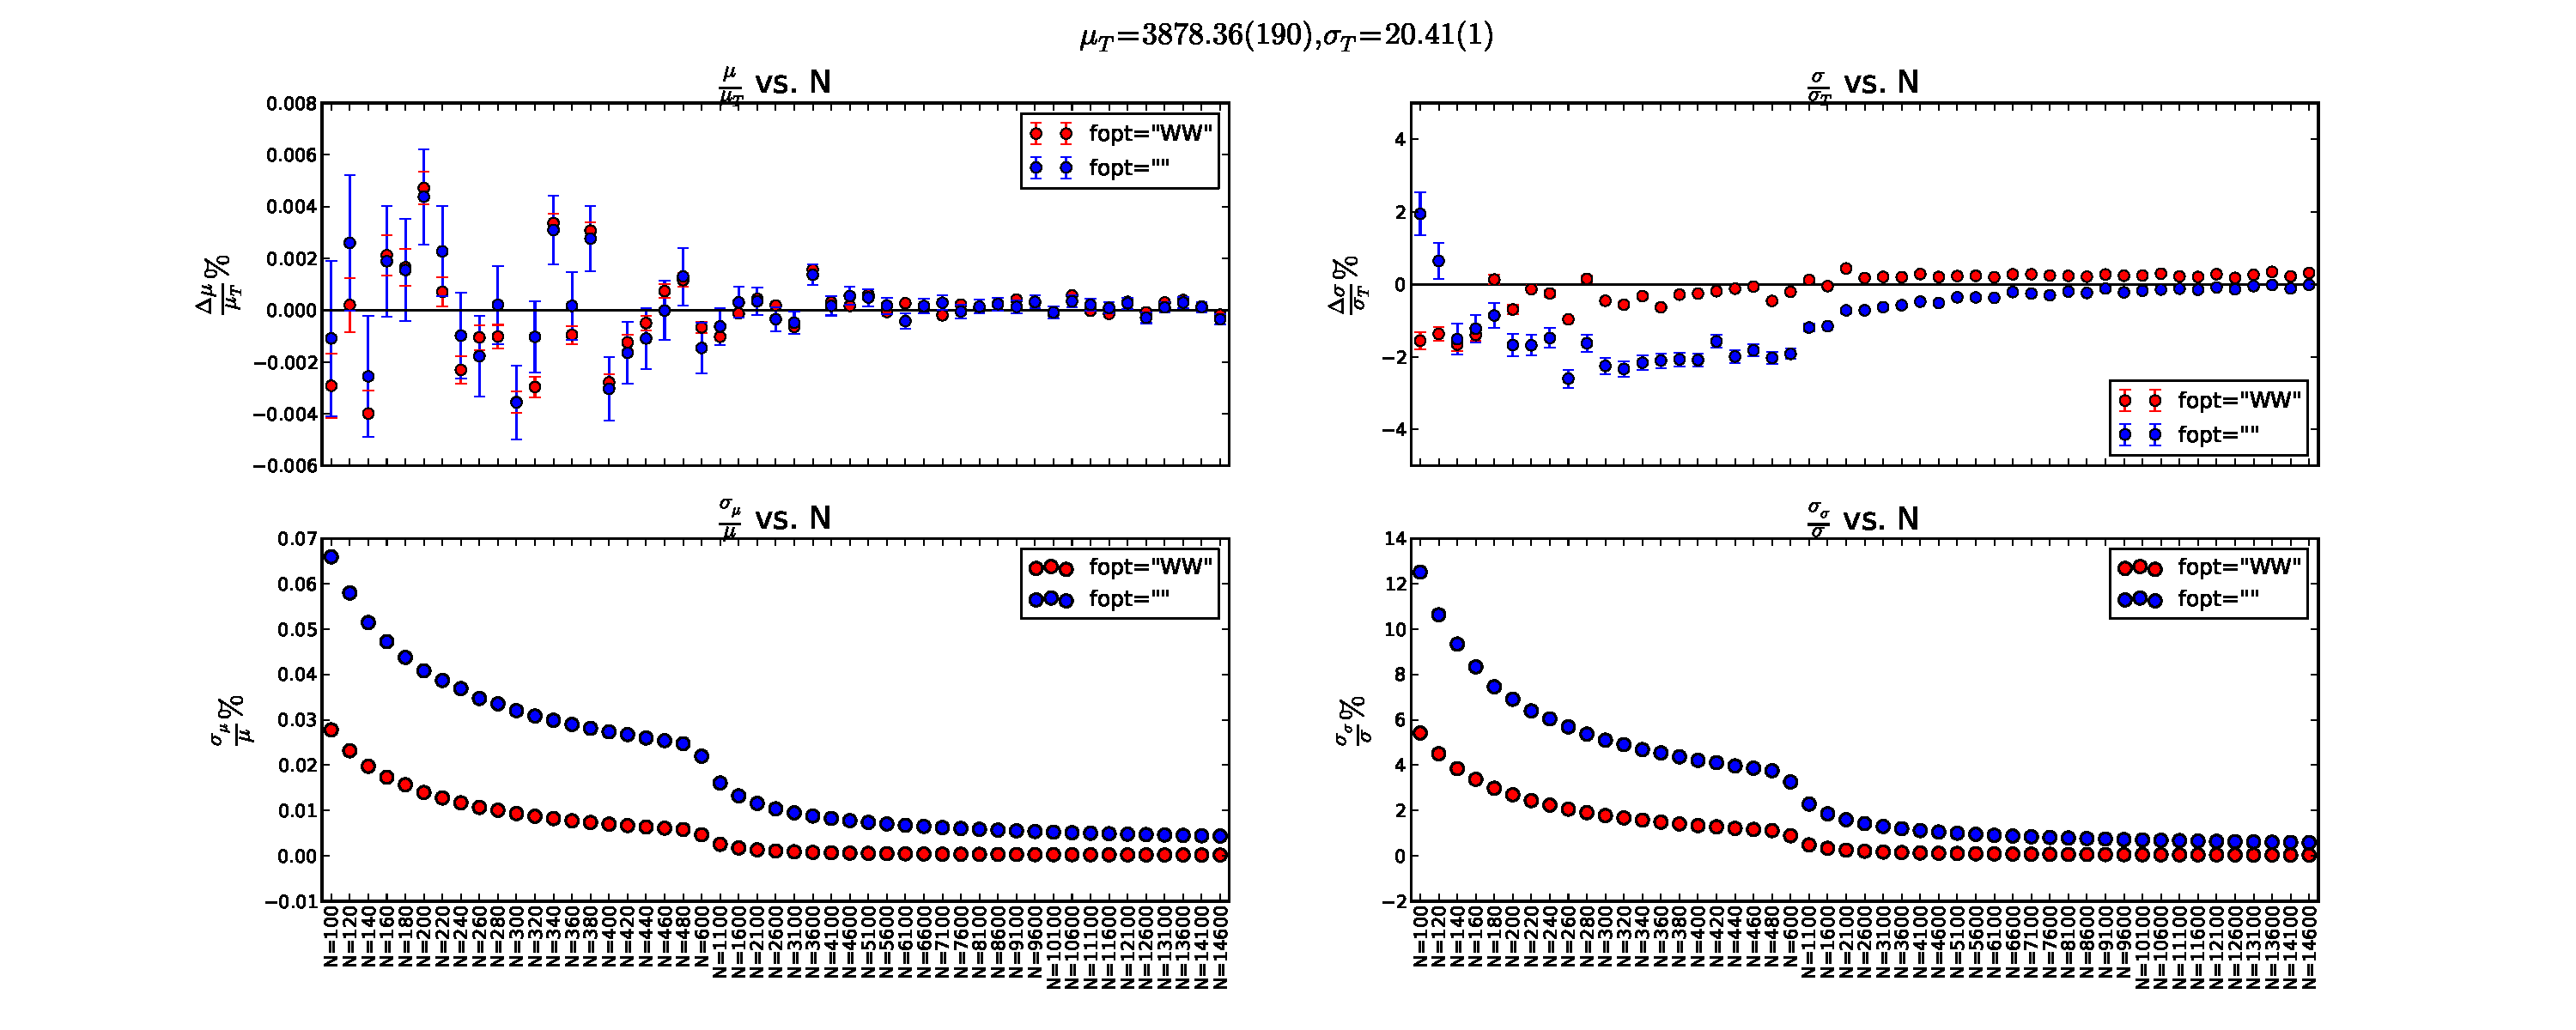
\includegraphics[height=2.5in,width=5.5in]{fit-comp_MU-190_SG-1_fit-opt-WW_binw-025.pdf}
	%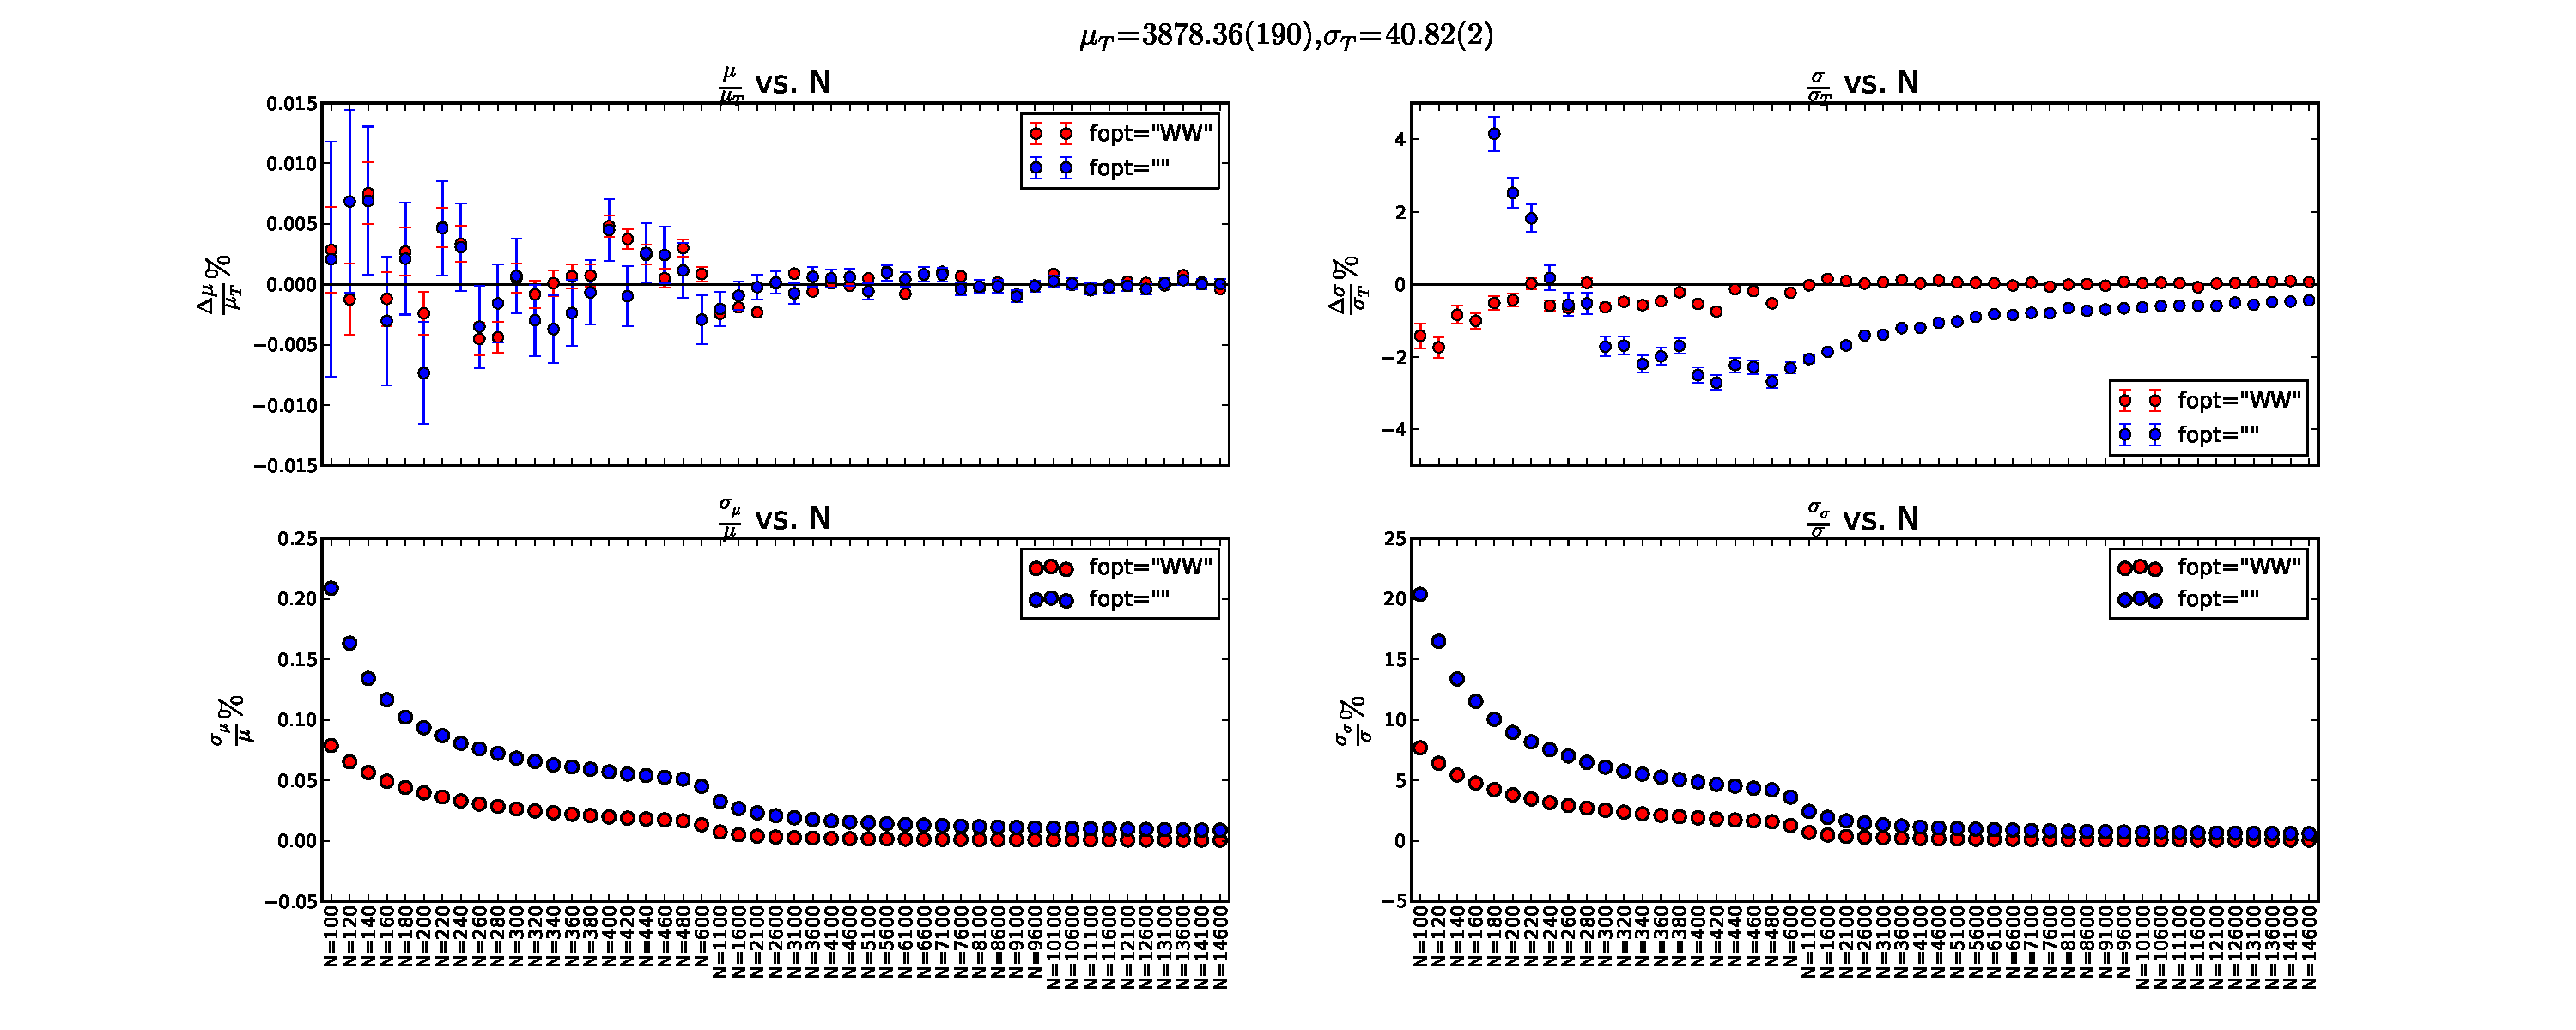
\includegraphics[height=2.5in,width=5.5in]{fit-comp_MU-190_SG-2_fit-opt-WW_binw-025.pdf}
	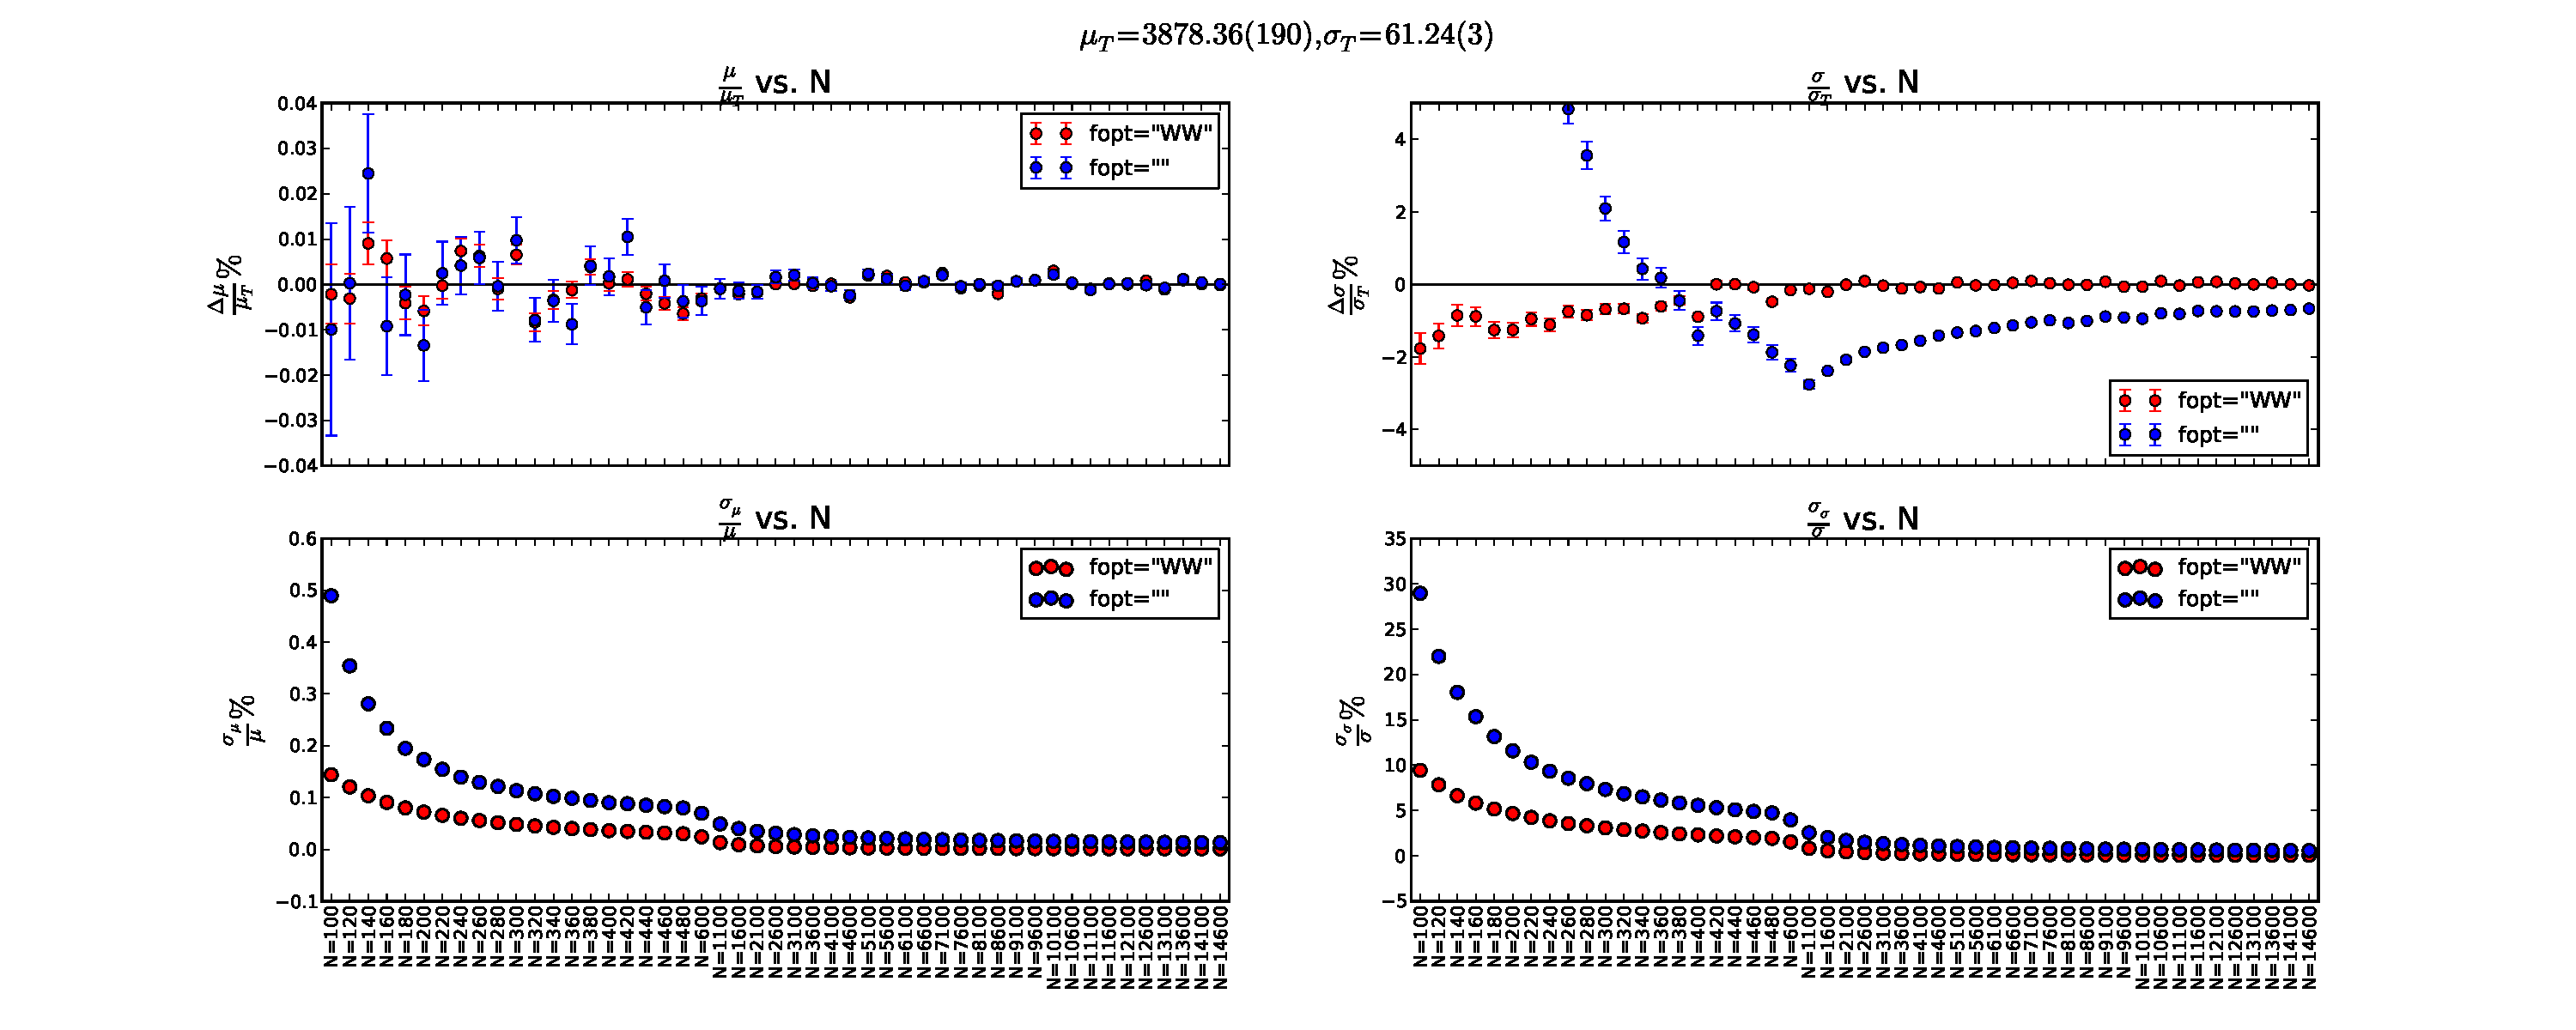
\includegraphics[height=2.5in,width=5.5in]{fit-comp_MU-190_SG-3_fit-opt-WW_binw-025.pdf}
	%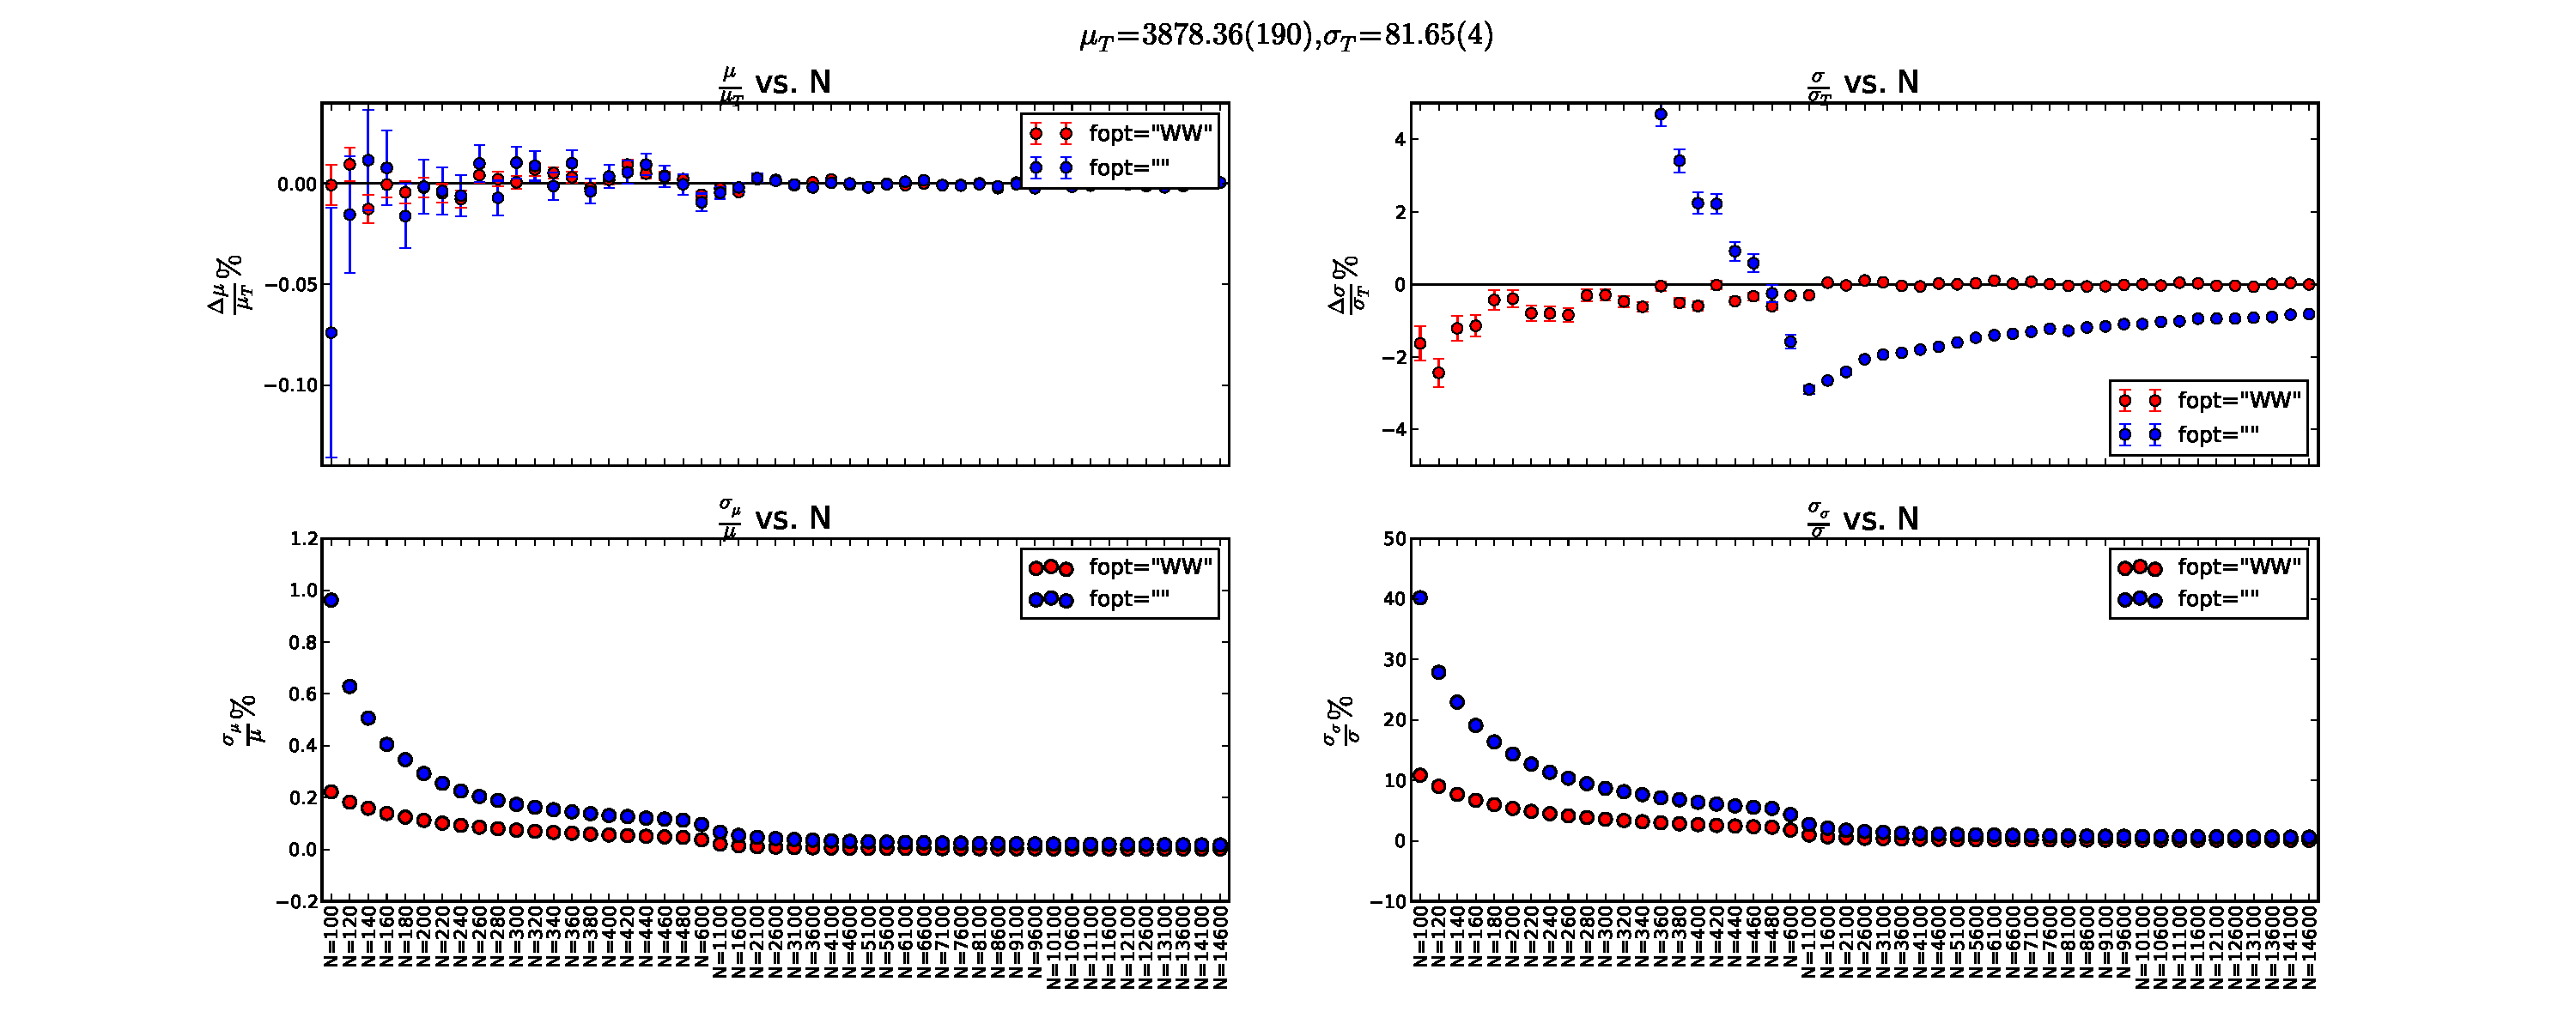
\includegraphics[height=2.5in,width=5.5in]{fit-comp_MU-190_SG-4_fit-opt-WW_binw-025.pdf}
	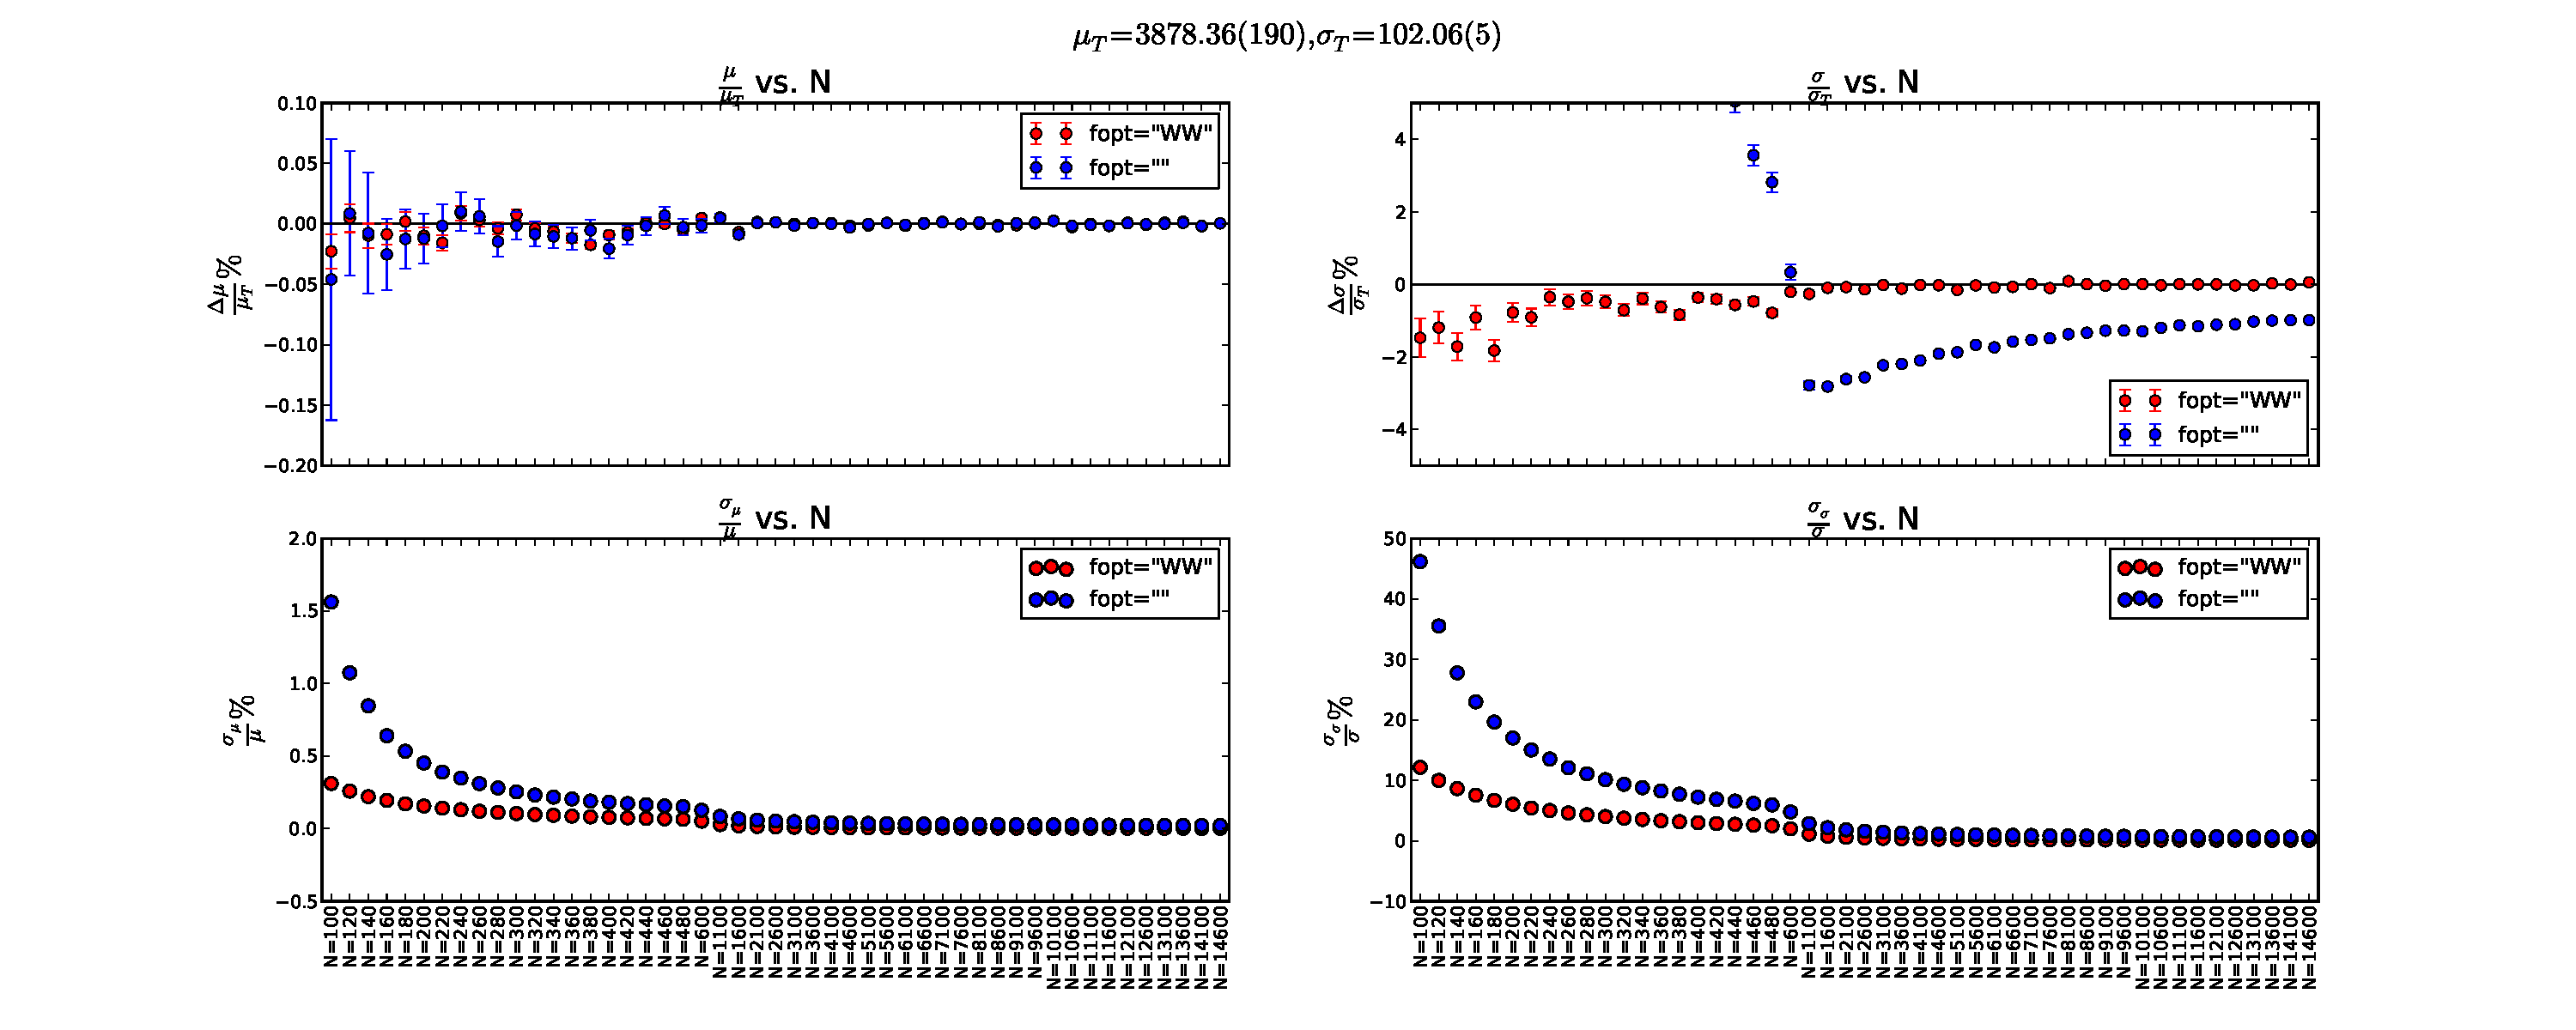
\includegraphics[height=2.5in,width=5.5in]{fit-comp_MU-190_SG-5_fit-opt-WW_binw-025.pdf}
	\caption{Extracted parameters (CSQWW and CSQ)as a function of N and $\sigma_{T}$}
	\label{fig3}
\end{figure*}

\clearpage

Following is a summary of the different ROOT Fit methods compared and their performance in the low statistical limit:

\begin{itemize}
	\item CSQ: Unacceptable
	\item MLE: Significantly better than CSQ, however, underestimates $\sigma_{T}$ by $\approx$ 1\%, and is susceptible to ``outliers''.
	\item CSQ-WW: Slightly more biased than MLE (underestimates $\sigma_{T}$ by $\approx$ 2\%) and the error on this estimate is lower than that of MLE. It is, however, not susceptible to ``outliers''.
\end{itemize}

Therefore, given the low statistics and the need to efficiently optimize the automation program during the production of a large scale system, it was best to use the CSQ-WW method, even though the statistical errors on the estimated $\sigma_{T}$ appear to be underestimated. 

This underestimation of the statistical errors by the finally used CSQ-WW method on the extracted time resolution, however, did not have a significant impact on the error on the time resolution we obtained during the production phase. This is because the final result is obtained by averaging the measured resolution over several points along the length of the bar and in the process the contribution of the statistical error from each point is greatly reduced. 

\textit{I have 2 figures that can support the above statement, that I am going to show in Figures 4 and 5 and after discussion with the group, will refine the one we agree upon to publish}

Fig. 4 shows the statistical errors for the length-averaged time resolution for various bar lengths using production data (\textit{and therefore using only CSQ-WW; I should do refit production data with CSQ and MLE to complete this plot})
\begin{itemize}
 	\item \textit{source: Production data:Normal ordering:CSQ-WW $\langle res\_2\_3\_4 \rangle$}
 	\item \textit{I should do the same for CSQ and MLE}
 \end{itemize}

\begin{figure*}[ht]
	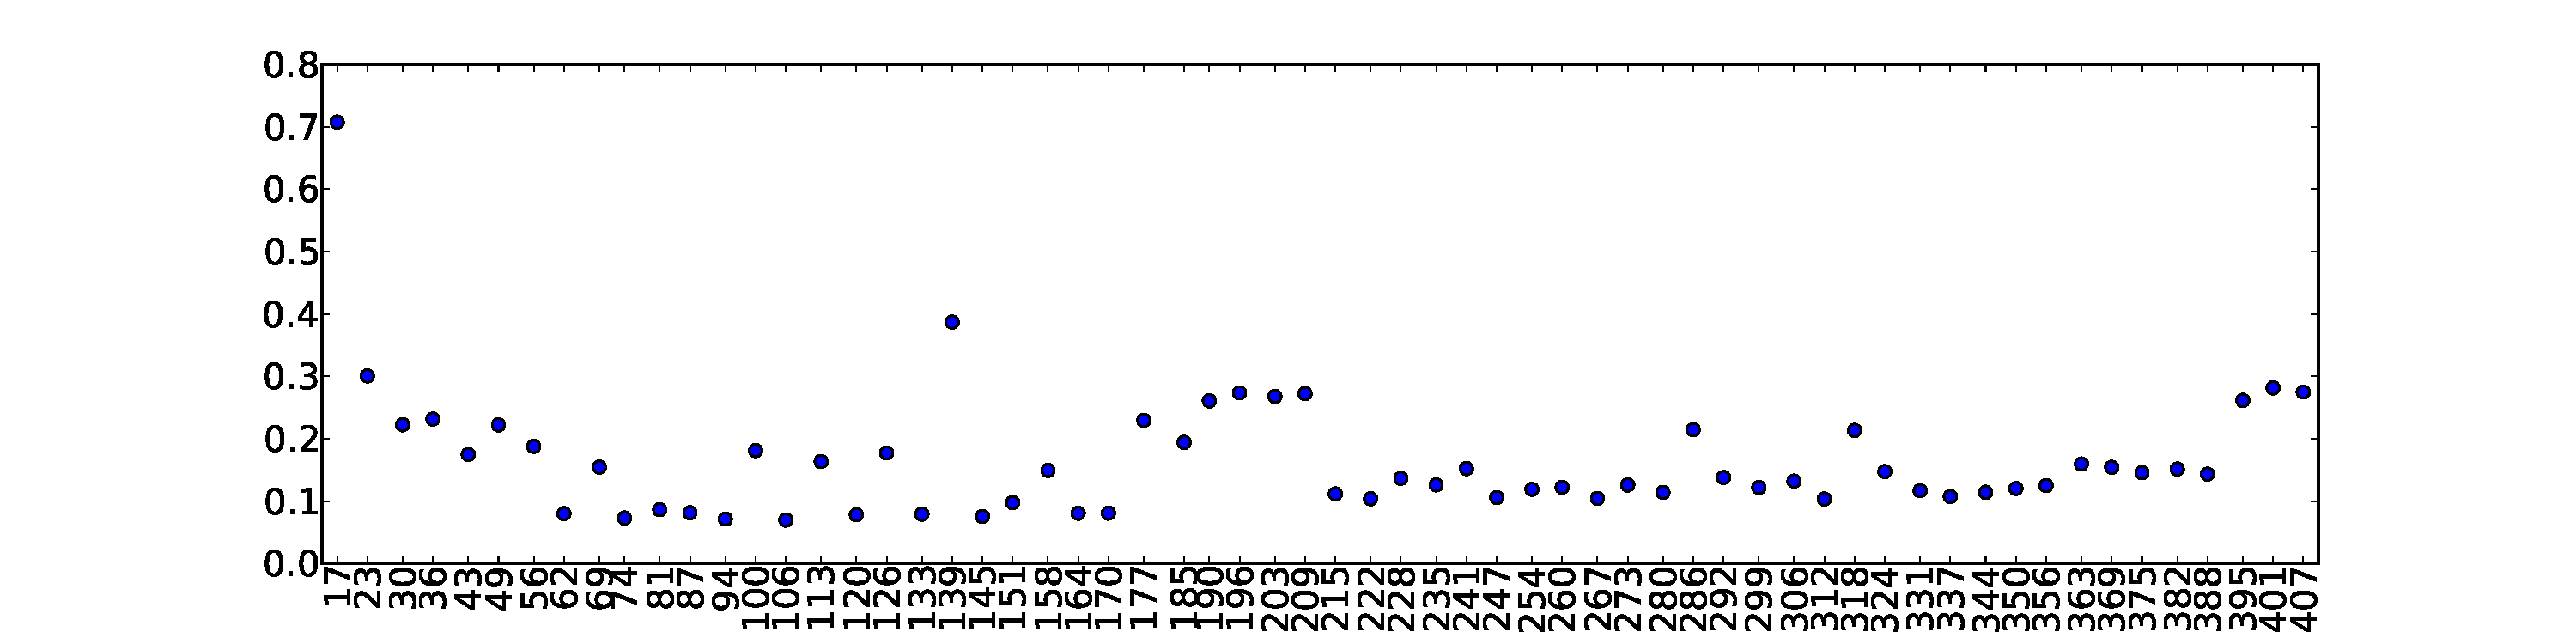
\includegraphics[height=2.5in,width=5.5in]{err_res_2_3_4_pointXX_cont.pdf}
	\caption{$\sigma_{\langle res\_2\_3\_4 \rangle}$ vs bar length}
	\label{fig4}
\end{figure*}

Fig. 5 shows the length-avaraged time resolution for 3-bar combination 2-3-4 from the production data($\langle res\_2\_3\_4 \rangle$), but after re-analysis and comparing all the different fit methods. The point of this plot is to mainly show that the ``Propaganda plot flucations'' are beyond the statistical fluctuations that could be estimated during the production phase and to additionally note the reason for using CSQ-WW in stead of CSQ and MLE. Note, the effect of the bin-width on the CSQ-WW method fits. Also keep in mind, there are some caveats to this plot, all for CSQ data points, for sometimes the fits failed or returned very biased resolutions (which is to be expected for now N and especially when bin-width=0.25) and those points were removed from the analysis. 

\begin{figure*}[ht]
	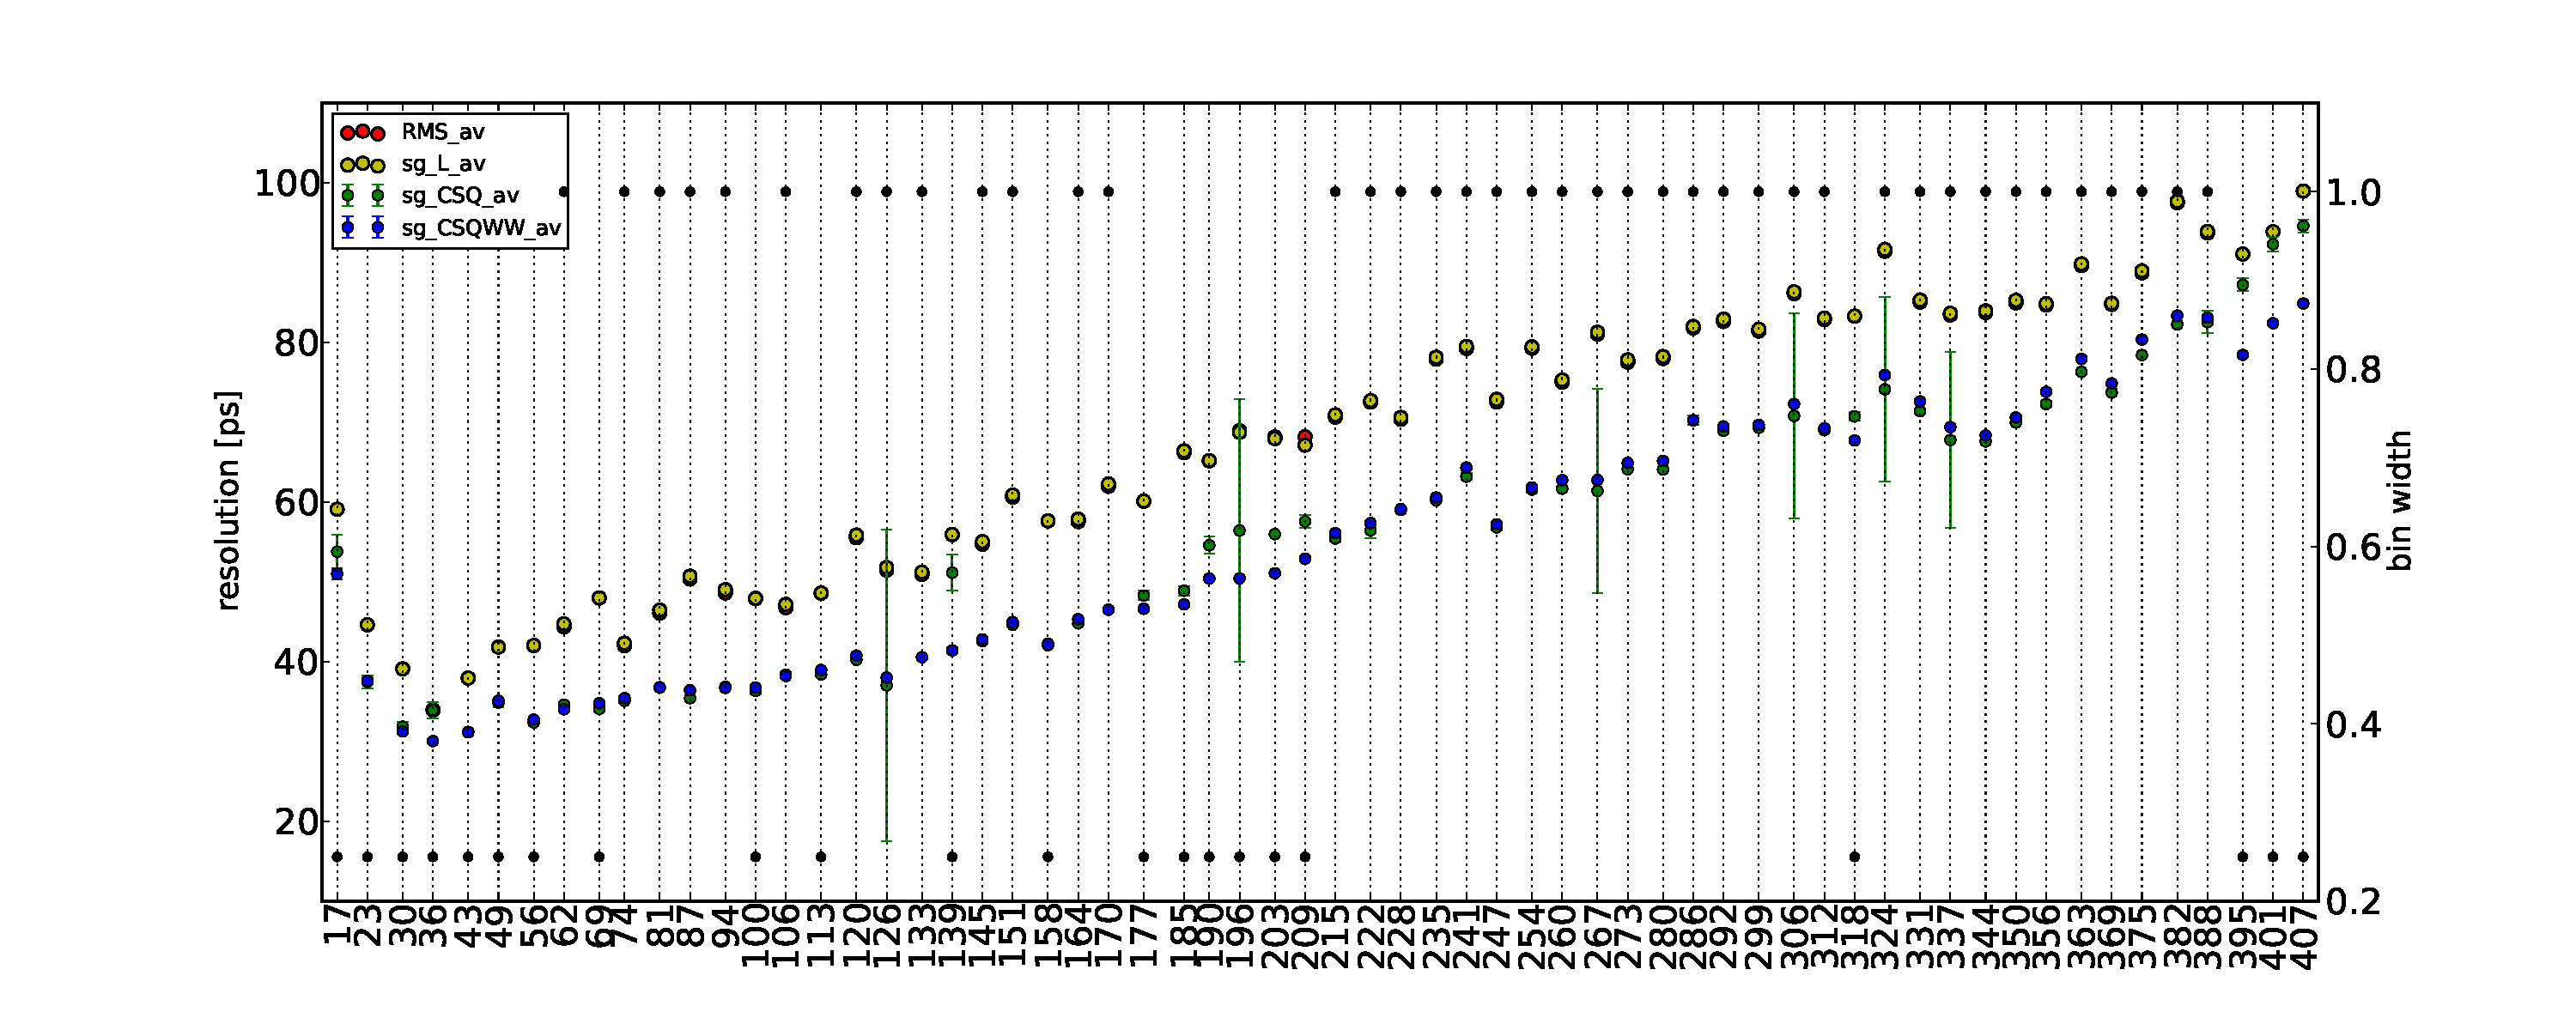
\includegraphics[height=4in,width=6in]{bar_stats_averages.pdf}
	\caption{ $\langle res\_2\_3\_4 \rangle$ re-analyzed using all fitting techniques}
	\label{fig5}
\end{figure*}

The only impact of using the underestimated errors of CSQ-WW is in the interpretation of the time resolution versus point-along-the-bar plot, where the underestimated errors may lead to the interpretation that the fluctuation of the data points is beyond what can be explained statistically. In order to bring out this underestimation, Figure 6. shows a plot for the resolution vs. point using CSQ, MLE and CSQ-WW for N and $\sigma_{T}$ where all methods return similar results. Here it can be seen that the results from CSQ-WW underestimate the errors, especially relative to MLE and CSQ.

\begin{figure*}[ht]
	
\includegraphics[height=2.5in,width=5.5in]{placeholder.pdf}
	\caption{Demo underestimation of errors by CSQWW by comparing with MLE by way of resolution vs. point plot (I had previously compared with CSQ, but with binw=0.25, CSQ is no longer valid to compare with if sets with binw=0.25 is to be used) }
	\label{fig4}
\end{figure*}  

\clearpage

\clearpage

\subsection{Effect of error on estimated Time Walk parameters on the time resolution is not determined}
For each 2-day measurement the Time Walk (TW) parameters are estimated (\textit{ref. to sec. in pub.}) and are used to correct each of the TDC measurements for TW (\textit{ref. to formula in pub.}) that go into calculating T (\textit{ref. to formula in pub.}). The error in the estimated TW parameters -- which apart from being statistical can also include non-statistical effects that can vary between measurements --, however, is not accounted for by the width of this T distribution. The only way to estimate the effect of the error of the estimated TW paramaters is to make several 2-day measurements and study the distribution of the respective time resolution measurements. This procedure will be described in detail in the relevant section.

\subsection{Non-statistical sources of error are not determined}
\textit{
\begin{itemize}
	\item Variation of physical paramaters of counters: Scintillators and PMTs
\end{itemize}
}

\subsection{Summary}
To summarize, the error on the time resolution obtained during the production phase could not possibly account for all possible sources of error, statistical and non-statistical. The errors obtained during the production phase and their limitations, especially in regard to some key plots, like resolution vs. length and in interpreting the ``fluctuations in the propaganda'' were discussed. It was found that the ``fluctuations in the propaganda'' cannot be explained by the statistical errors estimated in the production phase (section 1.1) and errors from effects described in sections 1.2 and 1.3, that were unaccounted for during the productin phase, will have to be estimated in a post production study of the error estimate. The rest of the section deals with a detailed discussion of this study and the results from therein.

\end{document}